\documentclass[11pt]{article}

\usepackage[margin=1in]{geometry}
\usepackage{amsmath,amssymb,amsthm,mathtools}
\usepackage{booktabs}
\usepackage{capt-of}
\usepackage{enumitem}
\usepackage{microtype}
\usepackage{tikz}
\usetikzlibrary{decorations.pathmorphing,patterns,arrows.meta,positioning}
\emergencystretch 1em
\usepackage[colorlinks=true,linkcolor=blue,citecolor=blue,urlcolor=blue]{hyperref}

\theoremstyle{plain}
\newtheorem{theorem}{Theorem}[section]
\newtheorem{proposition}[theorem]{Proposition}
\newtheorem{lemma}[theorem]{Lemma}
\newtheorem{corollary}[theorem]{Corollary}

\theoremstyle{definition}
\newtheorem{definition}[theorem]{Definition}
\newtheorem{example}[theorem]{Example}

\theoremstyle{remark}
\newtheorem{remark}[theorem]{Remark}

\newcommand{\GammaSet}{\Gamma_{\mathrm{set}}}
\newcommand{\GammaEff}{\Gamma_{\mathrm{eff}}}
\newcommand{\GammaB}{\Gamma_{\mathcal B}}
\newcommand{\eps}{\varepsilon}

\title{Algorithms and Certificates for Finite Effective Causal Descent:\\
Width-Based Synthesis for Sensor-Limited Mechanical Control}
\author{Anonymous}
\date{}

\begin{document}
\maketitle

\begin{abstract}
Finite decision systems under partial observation face a simple obstruction: a
controller cannot choose different actions in scenarios that its sensors do not
distinguish.  This article develops the finite algorithmic companion to
effective causal descent: a proof-producing synthesis pipeline for finite
sensor-limited mechanical models.  A finite presentation consists of policy variables, finite domains, and
explicit local relations; global policies are exactly the assignments satisfying
all relations.  Effectivity and bounded realisability are represented by finite
implementation catalogues, costs, and budgets.  The main algorithmic layer is a
certificate-producing dynamic program over tree decompositions, with ordinary
and weighted-width bounds, independently checkable message tables, and typed
certificates for policies, refutations, optimum costs, fibre conflicts, sensor
repairs, finite-element rows, and sparsification ladders.  The mechanics layer
converts declared structural models with rational data into certified exact
influence rows, and turns certified affine response rows into inner and outer
finite ECD models, proving the sound sandwich
\(\Gamma(P^-)\subseteq\Gamma(P^{\mathrm{true}})\subseteq\Gamma(P^+)\).
Width-adaptive sparsification gives monotone certified refinement rather than a
performance claim.  A recorded computational study executes a mechanics
benchmark suite over truss and mass-spring families with quantised-sensor
observation variants, a width-adaptive sparsification study over retained-scope
ladders, and a comparative scaling study of the certified pipeline against
external SAT, CP-SAT, and MILP solvers on identical mechanics-derived
instances; a version-exact replication reproduces the recorded comparative
study, and a dense-family extension to seventeen and eighteen actuators
records the certificate-growth and memory boundary of the pipeline; all
limits, relation-table boundaries, and unresolved brackets are
reported explicitly.  An exact two-spring demonstrator and a finite prototype
artifact exercise the certificate grammar, reject corrupted certificates, and
produce controlled-width benchmark reports.  In every external comparison, an
answer is accepted only when cross-checked by an independently verified native
certificate, and timeouts, missing solvers, and solver statuses without a
certified claim remain inconclusive.
\end{abstract}

\noindent\textbf{Keywords:} finite effective causal descent; sensor-limited control;
certifying algorithms; tree decompositions; weighted width; finite-element
certification; sparsification; independent verification.

\tableofcontents

\section{Introduction}
\label{sec:introduction}

A mechanically admissible response need not be implementable by a controller
whose observations fail to distinguish the situations requiring different
actions.  A load case, damage state, or inspection record may determine which
actions are safe, while the available sensor readings merge several such cases
into one information state.  Once the information state is fixed, the controller
has only one command available.  The first task is therefore not to solve a
continuous mechanics problem in full generality, but to certify the finite
relation between observations, admissible actions, and implementable policies in
a declared model.

This article develops the finite, proof-producing side of effective causal
descent (ECD).  The foundational monograph (version~46) supplies the presentation-relative
language: local validity, compatibility of a diagram, effective realisability,
and bounded realisability.  Here we specialise that language to explicit finite
instances and to mechanically generated finite relations.  The guiding rule is:
\emph{topological order is the constraint; feasibility is the priority}.  We
first fix the finite input representation, then the certificate grammar, then
the one-shot fibre and sensor-repair theory, then the solver and verifier,
then the mechanical relation generator, then the sparsification and benchmark
layers.  Comparative performance claims come last
and require experiments; they are not consequences of the structural theory.

The contribution is organised around certificates.  A successful run should
return a policy that an independent verifier checks.  A negative run should
return a refutation certificate, not merely a solver log.  A mechanical row
should carry the numerical or exact-arithmetic evidence justifying its safe,
unsafe, or unresolved status.  A sparsified instance should come with interval
bounds proving the appropriate inner--outer inclusions.  The computational
statuses are deliberately limited: certified satisfiable, certified
unsatisfiable, certified optimal, or inconclusive.  The design follows the
certifying-algorithms discipline: every output is checkable evidence, not a
trusted narrative~\cite{mcm11}.

The finite contributions are the following.  First, we fix an explicit input
schema for finite ECD presentations and implementation catalogues.  Second, we
specify typed certificates that an independent verifier can check.  Third, we
prove one-shot fibre conflict bounds, reachability-correct causal compilation,
and explicit-table complexity boundaries.  Fourth, we give a width-based dynamic
program with weighted-width accounting and message-table certificates.  Fifth,
we characterise one-shot sensor repair exactly as a hitting-set condition on
inclusion-minimal conflict cores, and prove the design side hard:
minimum-cardinality repair from a listed candidate family is NP-complete and
W[2]-hard in the number of added sensors.  Sixth, we connect exact affine mechanical
rows to finite inner and outer ECD models.  Seventh, we prove a monotone
sparsification ladder for retained scopes.  Eighth, we convert declared
structural models with rational data into certified exact influence rows whose
base states are verified by exact residual substitution.
Finally, we report an artifact that exercises these certificates, rejects
corrupted evidence, and produces controlled-width benchmark summaries; the
recorded mechanics study executes a benchmark suite with quantised-sensor
observation variants, a sparsification ladder study measuring the
width--inconclusiveness tradeoff, and a comparative scaling experiment against
external solvers on identical instances, without claiming external-solver
superiority.

\subsection*{Relation to prior work}

The machinery is assembled from established lines.  Acyclic join processing
supplies the width-zero regime~\cite{yannakakis81}; width-directed consistency
and decomposition supply the bounded-width
regime~\cite{freuder82,dechter03,bodlaender-koster08}; the
certifying-algorithms discipline requires outputs that carry checkable
evidence~\cite{mcm11}; parameterised complexity calibrates what width-bounded
computation cannot achieve~\cite{downey-fellows99,impagliazzo-paturi01}.
The source problem is posed by the decentralised-control tradition: synthesis
and decision making under nonclassical information
structures~\cite{witsenhausen71,papadimitrioutsitsiklis86,bernstein02}.
Sensor-selection studies budget observations for information
value~\cite{krauseguestrin07}, and nested-dissection eliminations price
fill-reducing orders on meshes~\cite{george73,liptontarjan79}.  None of these
lines supplies the assembly this article reports: typed certificates for
finite ECD instances --- negative answers as verified refutations rather than
solver logs, sensor repair as a hitting-set certificate, mechanical rows as
exact-arithmetic evidence, and sparsification as verified inner--outer
inclusions --- under a status discipline that records inconclusive outcomes
instead of discarding them.  The engines are classical; the assembly and its
recorded execution are the contribution.

\section{Finite ECD presentations}
\label{sec:finite-presentations}

\begin{definition}[Finite ECD presentation]
A finite ECD presentation is a tuple
\[
  \mathcal P=(X,(D_x)_{x\in X},(S_i,R_i)_{i\in M}),
\]
where \(X\) is a finite set of policy variables, each \(D_x\) is a finite
nonempty domain, each scope \(S_i\subseteq X\) is finite, and
\[
  R_i\subseteq\prod_{x\in S_i}D_x
\]
is an explicitly represented permitted table.  Its global policy space is
\[
  \Gamma(\mathcal P)=
  \{a\in\prod_{x\in X}D_x: a|_{S_i}\in R_i\text{ for all }i\in M\}.
\]
\end{definition}

In a sensor-limited mechanics model, a variable often has the form \((j,o)\),
where \(j\) is an actuator or decision channel and \(o\) is an information state
produced by the available sensors.  The finite relation tables record which
joint commands are certified safe for each scenario or local mechanical
constraint.

\begin{definition}[Canonical finite input]
\label{def:canonical-input}
The verifier-facing input convention is
\[
I=(X,(D_x)_{x\in X},(S_i,R_i)_{i\in M},O,\operatorname{obs},
\mathcal L,c,B).
\]
Here \(X\), \(D_x\), \(S_i\), and \(R_i\) give the explicit finite relation
instance; \(O\) records observation states and
\(\operatorname{obs}:W\to O\) records the map from a finite scenario set \(W\),
or from histories, to information states when those data are relevant;
\(\mathcal L\) is an optional finite implementation catalogue; \(c\) is its cost
map; and \(B\) is an optional budget.  If a table is replaced by a succinct
circuit, automaton, or finite-element generator, the input representation has
changed and the corresponding complexity or soundness claim must be restated for
that source representation.
\end{definition}

\begin{definition}[Finite implementation catalogue]
For controller \(j\), let \(\mathcal L_j\) be a finite catalogue of
implementations with evaluation map \(\operatorname{eval}_j(\ell,o)\), defined
on the controller's information states \(o\in O_j\), and cost \(c_j(\ell)\).  Introduce implementation variables
\(\ell_j\in\mathcal L_j\cup\{\bot\}\), where \(\bot\) is compatible with every
behavioural assignment and has infinite cost.  A finite-cost catalogue policy is
one satisfying
\[
  x_{j,o}=\operatorname{eval}_j(\ell_j,o)
  \qquad(o\in O_j)
\]
with every \(\ell_j\ne\bot\).
\end{definition}

Thus finite set-theoretic existence is separated from existence in a declared
implementation catalogue, and budgeted existence is separated again by a cost
bound.  This is the finite analogue of the nested spaces
\(\GammaSet\supseteq\GammaEff\supseteq\GammaB\), but it is entirely explicit.

\begin{proposition}[Finite effective collapse]
\label{prop:finite-collapse}
Let \(\mathcal P\) be a finite ECD presentation whose variables carry the form
\(x_{j,o}\), where \(j\) ranges over a finite set of controllers with
information states \(o\in O_j\), the variables of each controller sharing a
domain \(D_j\).  Equip each controller with the unrestricted catalogue
\(\mathcal L_j\) of all total functions \(O_j\to D_j\), evaluated by
\(\operatorname{eval}_j(\ell,o)=\ell(o)\).  Then every policy
\(a\in\Gamma(\mathcal P)\) is a catalogue policy, so set-theoretic and
unrestricted-catalogue existence coincide.
\end{proposition}

\begin{proof}
Every catalogue policy is in particular an assignment satisfying every row,
so catalogue existence implies set-theoretic existence.  Conversely, given
\(a\in\Gamma(\mathcal P)\), put \(\ell_j(o)=a_{j,o}\) for \(o\in O_j\);
then \(\ell_j\in\mathcal L_j\) and
\(a_{j,o}=\operatorname{eval}_j(\ell_j,o)\) for every \(o\), so \(a\) is a
catalogue policy with every \(\ell_j\ne\bot\).
\end{proof}

\begin{remark}[What the collapse separates]
\label{rem:collapse-separates}
The collapse confines the finite analogue of
\(\GammaSet\supseteq\GammaEff\supseteq\GammaB\): under unrestricted catalogues
the set-theoretic and effective questions coincide, and the remaining
separations are the declared-catalogue and budget separations of
Definition~\ref{def:canonical-input}.  A bounded class retains content only
after the bound is declared --- controller memory, representation size, or
cost budget.  Existence is thereby separated from the cost of finding it: a
synthesis timeout or a table-size limit is inconclusive, not evidence of
non-existence, which is the status discipline of
Section~\ref{sec:certificates}.
\end{remark}

\begin{remark}[Value costs and catalogue costs]
\label{rem:costs}
Two cost notions coexist and must not be conflated.  The catalogue cost map
\(c\) of Definition~\ref{def:canonical-input} prices implementations
\(\ell\in\mathcal L_j\).  Optimum certificates instead use value costs: a
costed instance additionally carries nonnegative rational value costs
\(\kappa_x(v)\) for \(x\in X\) and \(v\in D_x\), and the cost of an
assignment is
\[
  \kappa(a)=\sum_{x\in X}\kappa_x(a_x).
\]
The \texttt{DP-OPTIMUM} certificates introduced in
Section~\ref{sec:certificates} and developed in Section~\ref{sec:width-dp}
certify the minimum of \(\kappa\) over \(\Gamma(\mathcal P)\); the benchmark suite of
Section~\ref{sec:mechanics-benchmarks} uses per-actuator value costs with
\(\kappa_x(1)=1\) and \(\kappa_x(0)=0\), so its optima report the minimum
number of active actuators.
\end{remark}

\section{Certificate grammar and status discipline}
\label{sec:certificates}

The verifier accepts typed certificates rather than solver narratives.  The
grammar contains the following core forms.

\begin{center}
\begin{tabular}{@{}p{0.23\linewidth}p{0.41\linewidth}p{0.25\linewidth}@{}}
\toprule
Certificate & Data & Certified claim\\
\midrule
\texttt{POLICY} & total assignment to all variables & global section\\
\texttt{FIBRE-CONFLICT} & one observation fibre and excluded-action witnesses & no one-shot selector on that fibre\\
\texttt{SENSOR-REPAIR} & selected sensors and conflict cores & sensor sufficiency or optimality in a finite master problem\\
\texttt{TREE-DECOMP} & bags, edges, root, factor placement & valid decomposition\\
\texttt{DP-REFUTATION} & decomposition and message tables & no global assignment\\
\texttt{DP-OPTIMUM} & decomposition, message tables, root value & minimum finite cost\\
\texttt{FE-ROW} & response interval and row status & safe, unsafe, or unresolved finite row\\
\texttt{SPARSIFICATION-\allowbreak BATCH} & retained scopes and omitted-term bounds & inner and outer sparse model\\
\bottomrule
\end{tabular}
\end{center}

\begin{remark}[Status discipline]
\label{rem:status-discipline}
The implementation reports only four mathematical statuses:
\texttt{CERTIFIED-SAT}, \texttt{CERTIFIED-UNSAT}, \texttt{CERTIFIED-OPT}, and
\texttt{INCONCLUSIVE}.  A timeout, missing external solver, failed certificate
verification, or unresolved numerical row is inconclusive.  It is never a proof
of infeasibility.  The verification gate additionally emits bookkeeping
markers for the state of a gate check --- \texttt{VERIFIED},
\texttt{REJECTED}, \texttt{COMPLETE}, and \texttt{RELATION-TABLE-LIMIT} for
rows whose relation enumeration exceeds the recorded cap; these are harness
statuses, not answers, and the four mathematical statuses above are unaffected
by them.
\end{remark}

\section{One-shot fibres and causal compilation}
\label{sec:fibres-compilation}

The \texttt{FIBRE-CONFLICT} certificate type of the grammar rests on the
observation fibres.  Writing \(o=\operatorname{obs}\) for the observation map,
the observation fibre over an observation value \(z\in O\) is
\(o^{-1}(z)=\{w\in W:o(w)=z\}\): the set of scenarios that the available
observation map does not distinguish from one another.

\begin{theorem}[One-shot fibre criterion]
\label{thm:fibre-criterion}
Let \(o:W\to O\) be an observation map, let \(A\) be a finite action set, and
let \(S_w\subseteq A\) be the actions admissible in scenario \(w\).  An
observation-uniform action selector exists if and only if
\[
  A_z:=\bigcap_{w:o(w)=z}S_w\ne\varnothing
\]
for every realised observation value \(z\).  If a fibre fails, a certificate
using at most \(|A|\) scenarios in that fibre excludes every action, and the
bound is tight.
\end{theorem}

\begin{proof}
A selector chooses one action \(a_z\) for every observation value.  The action is
valid on the fibre over \(z\) exactly when \(a_z\in S_w\) for every scenario in
that fibre, equivalently \(a_z\in A_z\).  If \(A_z=\varnothing\), choose for each
action \(a\in A\) one scenario \(w_a\) in the fibre with \(a\notin S_{w_a}\).
The distinct chosen scenarios exclude all actions and have cardinality at most
\(|A|\).  Tightness is witnessed by \(S_{w_j}=A\setminus\{j\}\) for
\(A=\{1,\ldots,k\}\).
\end{proof}

\begin{theorem}[Reachability-correct forbidden-tuple compilation]
Consider a finite explicit history tree whose predictor nodes are partitioned
into information cells.  Introduce one policy variable for each information
cell.  For each unsafe leaf, read the information-cell/action labels along the
root-to-leaf path.  If the path requires the same information cell to take two
different actions, discard it.  Otherwise add the corresponding forbidden tuple.
The resulting finite presentation has global assignments exactly the policies
that avoid every unsafe leaf.
\end{theorem}

\begin{proof}
A path requiring two different actions at one information cell is unrealisable
by any observation-uniform policy, so it contributes no feasible unsafe
execution.  Every remaining unsafe path is reached precisely when the policy
matches all action labels on that path; forbidding the resulting tuple is
therefore exactly the condition that this unsafe leaf is not reached.
\end{proof}

\section{Finite complexity boundary}
\label{sec:complexity}

The explicit-table representation fixes the complexity claims.  The basic
frontier is standard finite CSP complexity, but it is important to state it in
the same encoding used by the verifier.

\begin{center}
\begin{tabular}{@{}p{0.62\linewidth}p{0.26\linewidth}@{}}
\toprule
Problem & Complexity\\
\midrule
Verify a proposed assignment & P\\
Unary constraints & P\\
Boolean binary constraints & P via 2-SAT\\
Boolean ternary explicit-table constraints & NP-complete\\
Binary disequality over a three-element domain & NP-complete\\
Nonexistence of a global assignment & coNP-complete\\
Counting global assignments & \(\#\mathrm P\)-complete\\
Minimum-cardinality fibre obstruction & NP-hard\\
Minimum-cardinality sensor repair (listed candidates) & NP-complete\\
\bottomrule
\end{tabular}
\end{center}

The hardness statements can be made under nonempty-local-relation promises, so
the obstruction is global compatibility rather than a locally empty factor.
These are not claims about arbitrary succinct generators.  Circuits, automata,
and finite-element preprocessors change the input representation and require
separate analysis.  Fixed-template dichotomy theorems, ETH (exponential-time
hypothesis) lower bounds, and parameterised hardness results should be cited only with their exact source
hypotheses and parameters; they are not universal classifications of finite ECD
presentations.  Appendix~\ref{app:reductions} records the encodings and the
standard reductions behind the table in the verifier-facing input format, and
cites the dichotomy, ETH, and W-hierarchy sources together with their exact
hypotheses~\cite{schaefer78,zhuk17,impagliazzo-paturi01,downey-fellows99}.
The design side of sensor repair is established directly rather than
transferred: deciding whether a listed candidate family contains a repairing
subfamily of at most \(k\) sensors is NP-complete, and the reduction
preserves the budget, so the problem is W[2]-hard under the parameterisation
by the number of added sensors (Proposition~\ref{prop:sensor-design-hardness}
and Appendix~\ref{app:reductions}).

The width boundary is identification-relative.  The primal graph of a finite
ECD presentation \(\mathcal P\) has vertex set \(X\), with an edge between
variables that occur together in a scope.

\begin{proposition}[Identification can destroy low width]
\label{prop:identification-width}
For every finite graph \(G\) there is a finite ECD presentation \(\mathcal P\)
and an identification of \(\mathcal P\) --- a partition of its variables into
blocks over a common domain, each block merged into one variable and each
table replaced by its image under the merge --- such that the primal graph of
\(\mathcal P\) is a disjoint union of edges and the primal graph of the
quotient presentation is \(G\).
\end{proposition}

\begin{proof}
For each edge \(uv\) of \(G\), take private variables \(u_{uv}\) and
\(v_{uv}\) over a common domain \(D\) and the full table \(D\times D\) on
\(\{u_{uv},v_{uv}\}\).  The scopes are pairwise disjoint, so the primal
graph is the matching of private copies.  Identify all copies of each vertex
of \(G\); every scope becomes an edge \(\{u,v\}\) of \(G\), and the full
tables merge to full tables, so the quotient presentation has primal graph
\(G\).
\end{proof}

\begin{remark}[Width is measured after identification]
\label{rem:identification-width}
The construction is the general form of the observation-variant convention of
Section~\ref{sec:mechanics-benchmarks}: the \texttt{split} variant keeps
command copies private, while the \texttt{same} variant identifies them, and
the recorded dense families realise the identified side, their scopes
covering the full actuator set, so the primal graph is complete.  Width
governs decomposition only after the identifications the interface enforces;
neither low mechanical-mesh width nor low width of a presentation of separate
scenario copies is sufficient by itself.  With a three-element domain and
disequality tables, the quotient is the graph-colouring instance of \(G\),
NP-complete in general~\cite{gareyjohnson79}, while the unmerged presentation
is a satisfiable matching of disequalities: width one before identification,
the width of \(G\) after it.
\end{remark}

\section{Width-based certifying dynamic programming}
\label{sec:width-dp}

Tree decompositions and their dynamic programs are
classical~\cite{robertson-seymour84,bodlaender93,bodlaender-koster08,arnborg-proskurowski89,dechter03};
the acyclic case is the join-tree regime of Yannakakis~\cite{yannakakis81}.
We fix the certificate-facing formulation.  Let \((T,(B_t)_{t\in T})\) be a
tree decomposition of the primal graph in which every variable occurs in at
least one bag (a variable occurring in no factor can be placed in the root
bag).  The solver orients \(T\) at a root \(r\), assigns each factor to a bag
containing its scope, and computes message tables from leaves to root.  For a
node \(t\), write \(T_t\) for the subtree rooted at \(t\),
\(V_t=\bigcup_{u\in T_t}B_u\) for its variables,
\(\Sigma_t=B_t\cap B_{\mathrm{pa}(t)}\) for its separator toward the parent
(with \(\Sigma_r=\varnothing\)), and \(F_t\) for the factors assigned to
\(t\).  Value costs \(\kappa\) are charged at the bag of each variable
closest to the root; the running-intersection property makes the bags
containing a variable connected, so the charging bag is well defined, and we
write \(\kappa_t(b)=\sum_{x\text{ charged at }t}\kappa_x(b_x)\).

\begin{lemma}[Private variables and factor separation]
\label{lem:private-variables}
If \(x\in V_t\setminus\Sigma_t\), then \(x\) occurs only in bags of \(T_t\).
Consequently, every factor whose scope meets \(V_t\setminus\Sigma_t\) is
assigned to a bag inside \(T_t\).
\end{lemma}

\begin{proof}
The bags containing \(x\) induce a connected subgraph of \(T\), and it
meets \(T_t\) because \(x\in V_t\).  If it also met the complement of
\(T_t\), a path between the two bags would cross the edge
\((t,\mathrm{pa}(t))\), so both \(B_t\) and \(B_{\mathrm{pa}(t)}\) would
contain \(x\), giving \(x\in\Sigma_t\) --- a contradiction.  For the second
claim, let factor \(i\) be assigned to a bag \(B_u\) with \(u\notin T_t\)
and suppose \(x\in S_i\cap(V_t\setminus\Sigma_t)\).  Factor containment
gives \(x\in S_i\subseteq B_u\), so \(x\) occurs in a bag outside \(T_t\),
contradicting the first claim.
\end{proof}

The message of a node \(t\) is the table \(\nu_t\), indexed by the
assignments \(s\) of the separator \(\Sigma_t\), with entries in
\(\mathbb Q_{\ge0}\cup\{\infty\}\) in cost mode and feasibility bits in
feasibility mode:
\[
  \nu_t(s)=\min\Bigl\{\,\sum_{x\in V_t\setminus\Sigma_t}\kappa_x(a_x)\ :\
  a\in\prod_{x\in V_t}D_x,\ a|_{\Sigma_t}=s,\ a|_{S_i}\in R_i\ \text{for
  every factor }i\text{ assigned in }T_t\,\Bigr\},
\]
the minimum over the empty set being \(\infty\); in feasibility mode the
entry records whether the set is nonempty.  The cost range is justified by
Lemma~\ref{lem:private-variables}: the variables of \(V_t\setminus\Sigma_t\)
occur only in bags of \(T_t\), so their charging bags lie in \(T_t\), while
the variables of \(\Sigma_t\) are charged at the parent or above and are
settled outside the message.  Messages are computed from leaves to the root
by the recurrence
\[
  \nu_t(s)=\min_{b}\Bigl(\kappa_t(b)+\sum_{c\in\mathrm{ch}(t)}
  \nu_c\bigl(b|_{\Sigma_c}\bigr)\Bigr),
\]
where the minimum ranges over the assignments \(b\) of \(B_t\) with
\(b|_{\Sigma_t}=s\) and \(b|_{S_i}\in R_i\) for all \(i\in F_t\); since
\(\Sigma_c=B_c\cap B_t\subseteq B_t\), the restriction \(b|_{\Sigma_c}\) is
well defined, and for a leaf the sum over children is empty.

\begin{lemma}[Recurrence correctness]
\label{lem:recurrence-correctness}
The recurrence computes, for every node \(t\), the message \(\nu_t\) defined
above.
\end{lemma}

\begin{proof}
By induction on the size of \(T_t\).  Fix an assignment \(s\) of
\(\Sigma_t\).  An assignment \(a\) of \(V_t\) extending \(s\) decomposes
uniquely into its restriction \(b\) to \(B_t\) and its restrictions to the
private parts \(V_c\setminus\Sigma_c\) of the child subtrees, and these
pieces recombine to a unique \(a\): the sets \(B_t\) and
\(V_c\setminus\Sigma_c\) partition \(V_t\), where a variable of
\(V_c\setminus\Sigma_c\) cannot lie in \(B_t\) without forcing membership
in \(\Sigma_c\) by connectedness, and sibling private parts are disjoint by
the same argument.  By Lemma~\ref{lem:private-variables}, a factor assigned
within \(T_t\) is either assigned at \(t\), in which case its scope is
contained in \(B_t\) and it constrains only \(b\), or it is assigned inside
some child subtree, in which case it is absorbed into that child's message.
The value costs split according to the charging bags.  The pieces are coupled
only through the separators \(\Sigma_c\), on which \(b\) prescribes values.
Hence the minimum over \(a\) factors into the displayed minimum over \(b\).
\end{proof}

For heterogeneous domains, the relevant state-space parameter is the weighted
width
\[
  \lambda(T)=\max_{t\in T}\sum_{x\in B_t}\lceil\log_2|D_x|\rceil.
\]
Every message table is indexed by assignments of a separator
\(\Sigma_t\subseteq B_t\), so it has at most \(2^{\lambda(T)}\) entries,
since \(\prod_{x\in B_t}|D_x|\le 2^{\lambda(T)}\).  Thus the
explicit-table recurrences run in
\(\operatorname{poly}(|I|,|T|)2^{\lambda(T)}\), up to indexing and
arithmetic factors.

\begin{proposition}[DP certificate soundness]
\label{prop:dp-soundness}
If an independent verifier recomputes all message tables of a
\texttt{DP-REFUTATION} certificate and obtains an infeasible root message,
then \(\Gamma(\mathcal P)=\varnothing\).  If it recomputes a \texttt{DP-OPTIMUM}
certificate with root value \(c<\infty\), then there is a global assignment
of value cost \(c\), and no assignment in \(\Gamma(\mathcal P)\) has lower value
cost for the declared finite instance.
\end{proposition}

\begin{proof}
The root has an empty separator, so by
Lemma~\ref{lem:recurrence-correctness} the root message aggregates over all
assignments of \(V_r=X\) subject to every factor --- exactly the global
policy space:
\[
  \nu_r()=\min_{a\in\Gamma(\mathcal P)}\kappa(a).
\]
An infeasible root message therefore certifies \(\Gamma(\mathcal
P)=\varnothing\), and a root value \(c<\infty\) certifies both that
\(\Gamma(\mathcal P)\ne\varnothing\) and that no global assignment has value
cost below \(c\).  The verifier recomputes every message table from the
decomposition and the instance data alone, so agreement at the root proves the
claim for the declared instance.
\end{proof}

\begin{remark}[A fixed-parameter reading]
\label{rem:fpt-reading}
The bound \(\operatorname{poly}(|I|,|T|)2^{\lambda(T)}\) is a fixed-parameter
tractability bound~\cite{downey-fellows99}: for the input consisting of the
instance together with its declared decomposition, both solving and
independently recomputing a \texttt{DP-REFUTATION} or \texttt{DP-OPTIMUM}
certificate (Proposition~\ref{prop:dp-soundness}) run in time exponential
only in the weighted width \(\lambda\).  The parameterised hardness of the
width programme sits on the design side instead: choosing a repairing sensor
family is W[2]-hard in the number of added sensors, already at width zero
(Proposition~\ref{prop:sensor-design-hardness}).  Evaluation width and design
budget are separate parameters, and the tractability boundary of the width
programme runs between them.
\end{remark}

\begin{example}[A hand-verifiable dynamic program]
\label{ex:dp-micro}
The recurrence, the charging rule, and both dynamic-programming certificate
types can be checked by hand on a four-variable instance.  Let
\(X=\{x_1,x_2,x_3,x_4\}\) with \(D_x=\{0,1\}\) for every \(x\), value
costs \(\kappa_x(1)=1\) and \(\kappa_x(0)=0\) as in the benchmark
convention of Remark~\ref{rem:costs}, and three pair factors
\[
  R_1=\{(0,1),(1,0),(1,1)\}\ \text{on}\ S_1=\{x_1,x_2\},
  \qquad
  R_2=\{(0,0),(1,1)\}\ \text{on}\ S_2=\{x_2,x_3\},
\]
\[
  R_3=\{(0,1),(1,0)\}\ \text{on}\ S_3=\{x_3,x_4\},
\]
read as \emph{at least one}, \emph{equality}, and \emph{exactly one}.  The
primal graph is the path \(x_1{-}x_2{-}x_3{-}x_4\).  A valid tree
decomposition is the path of bags
\[
  B_1=\{x_1,x_2\},\qquad B_2=\{x_2,x_3\},\qquad B_3=\{x_3,x_4\},
\]
rooted at \(r=B_3\), with factor \(i\) assigned to bag \(B_i\).  The
charging rule charges \(x_1\) at \(B_1\), \(x_2\) at \(B_2\) (its bag
closest to the root), and \(x_3,x_4\) at \(B_3\); the separators are
\(\Sigma_1=\{x_2\}\), \(\Sigma_2=\{x_3\}\), and \(\Sigma_r=\varnothing\).
The instance is small enough to check entirely by hand; it is a pedagogical
check of the recurrence and the certificate reading, not a recorded
artifact run.

The leaf message \(\nu_1\), indexed by the assignments of
\(\Sigma_1=\{x_2\}\), is
\[
  \nu_1(x_2{=}0)=1,\qquad \nu_1(x_2{=}1)=0:
\]
when \(x_2=0\) the factor \(R_1\) admits only the bag assignment
\((1,0)\), whose charge is \(\kappa_{x_1}(1)=1\), and when
\(x_2=1\) it admits \((0,1)\) and \((1,1)\), the cheaper being
\(\kappa_{x_1}(0)=0\); the sum over children is empty at a leaf.  The
message \(\nu_2\), indexed by \(\Sigma_2=\{x_3\}\), adds the charge of
\(x_2\), the only variable charged at \(B_2\):
\[
  \nu_2(x_3{=}0)=\kappa_{x_2}(0)+\nu_1(x_2{=}0)=0+1=1,
  \qquad
  \nu_2(x_3{=}1)=\kappa_{x_2}(1)+\nu_1(x_2{=}1)=1+0=1,
\]
since \(R_2\) forces \(x_2=x_3\).  At the root, \(R_3\) admits exactly the
bag assignments \((0,1)\) and \((1,0)\), both charged at \(B_3\):
\[
  \nu_r()=\min\bigl\{\kappa_{x_3}(0)+\kappa_{x_4}(1)+\nu_2(x_3{=}0),\;
  \kappa_{x_3}(1)+\kappa_{x_4}(0)+\nu_2(x_3{=}1)\bigr\}=2.
\]
Backtracking through the minimising entries yields the two optimal
sections \((1,0,0,1)\) and \((0,1,1,0)\); a brute-force sweep over the
sixteen assignments confirms that the global sections are exactly these
two and \((1,1,1,0)\), of value costs \(2\), \(2\), and \(3\).  Along the
root path each variable is charged exactly once --- \(x_1\) at \(B_1\),
\(x_2\) at \(B_2\), \(x_3\) and \(x_4\) at \(B_3\), totalling
\(1+0+0+1=2\) --- which is the non-double-counting guaranteed by
Lemma~\ref{lem:private-variables}.

The certificate reading is immediate.  The decomposition with its bags,
edges, root, and factor placement is a \texttt{TREE-DECOMP} certificate;
together with the three message tables and the root value \(2\) it
constitutes a \texttt{DP-OPTIMUM} certificate of value \(2\), and an
independent verifier recomputes \(\nu_1\), \(\nu_2\), and \(\nu_r\) from
the instance and the decomposition alone, as in
Proposition~\ref{prop:dp-soundness}.  In feasibility mode the same tables
carry bits, and the root bit records satisfiability.  Replacing the three
tables by
\[
  R_1'=\{(0,0),(1,0)\},\qquad
  R_2'=\{(0,1)\},\qquad
  R_3'=\{(0,0),(0,1)\}
\]
gives \(\nu_1'=(0,\infty)\) and \(\nu_2'=(\infty,0)\) (entries ordered by
the separator value \(0,1\)) and an infeasible root, since \(R_3'\)
forces \(x_3=0\) while \(\nu_2'(x_3{=}0)=\infty\); the same three tables
are then a \texttt{DP-REFUTATION} certificate, and indeed \(R_1'\) forces
\(x_2=0\), \(R_2'\) then forces \(x_3=1\), and \(R_3'\) forces
\(x_3=0\).  Finally, \(\lambda(T)=2\) here, since each bag holds two
Boolean variables, so every message table has at most
\(2^{\lambda(T)}=4\) entries; the separators are single variables, so the
displayed tables have two entries each.
\end{example}

\section{Sensor repair}
\label{sec:sensor-repair}

A sensor architecture is part of the presentation.  Fix one-shot data
\(W,o,A,(S_w)\) as in Section~\ref{sec:fibres-compilation}.  A conflict core
is a set \(C\subseteq o^{-1}(z)\) of scenarios within a single observation
fibre such that \(\bigcap_{w\in C}S_w=\varnothing\); it is inclusion-minimal
when no proper subset is a conflict core.  For a core \(C\), let
\[
  E_C=\{s:s\text{ is nonconstant on }C\}
\]
be the candidate sensors that separate scenarios of the core.  Adding a
sensor family \(T\) refines the observation map to
\(w\mapsto(o(w),(s(w))_{s\in T})\); the family repairs the one-shot problem
when the refined problem admits an observation-uniform selector.

\begin{theorem}[One-shot sensor repair]
\label{thm:sensor-repair}
\leavevmode
\begin{enumerate}
\item A sensor family \(T\) repairs the one-shot problem if and only if
\[
  T\cap E_C\ne\varnothing
\]
for every inclusion-minimal conflict core \(C\).
\item For any listed family of conflict cores, hitting every listed core is
necessary for repair, and it is sufficient --- hence exact --- when the list
contains all inclusion-minimal conflict cores.
\end{enumerate}
\end{theorem}

\begin{proof}
Necessity in (1).  Suppose \(T\cap E_C=\varnothing\) for a conflict core
\(C\subseteq o^{-1}(z)\).  Then every sensor \(s\in T\) is constant on
\(C\), so all scenarios of \(C\) share one refined observation value
\((z,v)\).  The refined fibre over \((z,v)\) contains \(C\), and its
admissible intersection is contained in \(\bigcap_{w\in C}S_w=\varnothing\).
By Theorem~\ref{thm:fibre-criterion} the refined problem admits no selector,
so \(T\) does not repair.

Sufficiency in (1).  Suppose some refined fibre \(F'\) fails, that is,
\(\bigcap_{w\in F'}S_w=\varnothing\).  All scenarios of \(F'\) share the
original observation value \(z\), so \(F'\) is itself a conflict core of
the original problem and, being finite and nonempty, contains an
inclusion-minimal core \(C_{\min}\).  Every sensor \(s\in T\) is constant
on \(F'\), hence on \(C_{\min}\), so \(T\cap E_{C_{\min}}=\varnothing\),
contradicting the hypothesis.  Hence every refined fibre has nonempty
admissible intersection, and Theorem~\ref{thm:fibre-criterion} yields a
selector for the refined problem.

Claim (2).  Necessity holds because a repairing family hits every core, by
the contrapositive of the necessity direction in (1).  When the list
contains all inclusion-minimal cores, hitting the list implies hitting every
inclusion-minimal core, which repairs by the sufficiency direction in (1);
conversely, a repairing family hits every core, in particular every listed
one.  Under this hypothesis the hitting-set condition is therefore exact for
one-shot repair.
\end{proof}

\begin{remark}[Minimal cores, not failing fibres]
\label{rem:cores-vs-fibres}
Hitting the sensors nonconstant on whole failing fibres is not sufficient for
repair.  A fibre may fail through a small core while the selected sensors
separate only scenarios outside that core; the refined fibre containing the
core then still fails.  Minimal failing fibres and inclusion-minimal conflict
cores differ in general: a minimal core need not exhaust its fibre, and a
failing fibre need not be minimal.  The exact objects for one-shot repair are
the inclusion-minimal conflict cores.
\end{remark}

The theorem separates two tasks: synthesising a policy for a fixed observation
architecture, and designing an observation architecture that makes policy
synthesis possible.  The second task contains hitting-set structure even when
the first task is easy.

\begin{proposition}[Sensor-design hardness]
\label{prop:sensor-design-hardness}
Deciding whether a listed family of candidate sensors contains a subfamily of
at most \(k\) sensors that repairs the one-shot problem is NP-complete, and
W[2]-hard under the parameterisation by \(k\).  Both statements hold already
for instances with one observation fibre and two actions, whose single-channel
presentations have one unary factor per scenario and an edgeless primal graph.
\end{proposition}

\begin{proof}
The decision problem lies in NP: a witness is the chosen subfamily together
with a selector for the refined problem, and a scan linear in the scenario
list checks the selector against every scenario.  For hardness, the set-cover
construction of Appendix~\ref{app:reductions} maps a covering instance with
budget \(k\) to a one-shot instance with one observation fibre and two
actions in which the inclusion-minimal conflict cores are exactly the pairs
\(\{w_0,w_j\}\) and a candidate sensor separates \(w_0\) from \(w_j\)
exactly when its covering set contains \(j\); by
Theorem~\ref{thm:sensor-repair}, the repairing subfamilies of size at most
\(k\) are exactly the covers of size at most \(k\).  The construction
preserves the budget, and set cover is W[2]-complete under the standard
parameterisation~\cite{downey-fellows99}, so the NP-hardness and the
W[2]-hardness both follow.  The single-channel presentation of the
constructed instance has one variable per observation value --- one, here ---
and one unary factor per scenario, an edgeless primal graph: the hardness is
present at width zero, and no decomposition of the declared instance removes
it (Remark~\ref{rem:fpt-reading}).
\end{proof}

\section{Certified affine mechanics front end}
\label{sec:mechanics-front-end}

The mechanics front end supplies finite relations; the finite solver certifies
policies or refutations for those relations.  For affine response rows,
\[
  y_i(a)=d_i+\sum_{x\in S_i}g_{ix}a_x,
\]
exact arithmetic or certified intervals classify each row as safe, unsafe, or
unresolved.  More generally, for a symmetric positive-definite discrete solve
\(Ku=f\), residual \(r=f-K\widehat u\), and certified lower spectral bound
\(\underline\lambda\le\lambda_{
\min}(K)\), one has
\[
  \|u-\widehat u\|_2\le \frac{\|r\|_2}{\underline\lambda},
  \qquad
  |c^T(u-\widehat u)|\le
  \|c\|_2\frac{\|r\|_2}{\underline\lambda}.
\]
Rows whose certified response intervals cross a threshold remain unresolved.

\begin{proposition}[Exact affine row certificates]
\label{prop:exact-affine-row-certificates}
For a finite affine response model with rational coefficients, finite actuator
domains, and a rational safety interval, exact rational evaluation produces
\texttt{FE-ROW} certificates whose safe rows form the corresponding finite ECD
relation table.  The verifier can recompute every row exactly.
\end{proposition}

\begin{proof}
For each action tuple, the response is a rational number obtained by a finite
sum of rational products.  The verifier recomputes this value, compares the
singleton response interval with the declared safety interval, and accepts the
row classification exactly when the comparison agrees.  The finite relation for
a mechanical scenario is precisely the set of action tuples whose certificates
verify as safe.
\end{proof}

\begin{proposition}[Inner--outer finite soundness]
\label{prop:inner-outer-soundness}
Let \(P^-\), \(P^{\mathrm{true}}\), and \(P^+\) be presentations sharing
variables, domains, and factor scopes.  If finite row certificates give
\[
  R_i^-\subseteq R_i^{\mathrm{true}}\subseteq R_i^+
\]
for every factor, then
\[
  \Gamma(P^-)\subseteq\Gamma(P^{\mathrm{true}})\subseteq\Gamma(P^+).
\]
Thus inner satisfiability gives a certified true finite-model policy, and outer
unsatisfiability gives a certified true finite-model refutation.  Inner
unsatisfiability with outer satisfiability is inconclusive.
\end{proposition}

\begin{proof}
Let \(a\in\Gamma(P^-)\).  For every factor \(i\),
\(a|_{S_i}\in R_i^-\subseteq R_i^{\mathrm{true}}\), so
\(a\in\Gamma(P^{\mathrm{true}})\).  The inclusion
\(\Gamma(P^{\mathrm{true}})\subseteq\Gamma(P^+)\) follows identically from
\(R_i^{\mathrm{true}}\subseteq R_i^+\).  Consequently, an assignment certified
by the inner model satisfies the true relations, so inner satisfiability
exhibits a true finite-model policy; if the outer model has no global
assignment, then neither has the true model, so outer unsatisfiability refutes
it; and when the inner model is unsatisfiable while the outer model is
satisfiable, both alternatives for the true model remain open, which is
recorded as inconclusive.
\end{proof}

\subsection{Declared structural models and certified influence rows}
\label{subsec:structural-front-end}

The affine models above can themselves be certified from declared structural
data.  A declared structural model consists of nodes with rational
coordinates and support flags, members with declared rational axial
stiffnesses, actuation patterns (node forces, or self-equilibrated axial
member pairs modelling pre-tension), load scenarios, and monitored linear
functionals (member forces or displacement components).  Members use rational
directions --- axis-aligned chords and 3-4-5 diagonals --- so every direction
cosine is rational and the assembled free-degree stiffness matrix \(K\) is
exact.  Two model kinds cover the families below: pin-jointed planar trusses
and grounded scalar mass-spring chains.

\begin{proposition}[Structural row certificates]
\label{prop:structural-row-certificates}
For a declared structural model with rational data, exact assembly and exact
rational solves produce, for every scenario and monitor, an affine row
\[
  y_i(a)=d_i+\sum_{x\in S_i}g_{ix}a_x
\]
with rational \(d_i\) and \(g_{ix}\), together with a certificate whose
base-state solves are checkable by exact residual substitution
\(K\widehat u=f\) against an independently assembled stiffness matrix, and
whose row data are checkable by regeneration.  The derived relation table is
exactly the set of actuator tuples whose row responses lie in the declared
safe interval.
\end{proposition}

\begin{proof}
Assembly accumulates rational dyads, so \(K\) is rational.  Exact
elimination over the rationals returns the unique solution of \(Ku=f\), and
the verifier proves it by substitution: \(K\widehat u-f=0\) exactly.
Monitors are rational linear functionals of \(u\), so \(d_i\) and every
\(g_{ix}\) are rational and recomputable, and the classification compares
the exact response with the declared rational interval.
\end{proof}

One structural distinction drives the benchmark families.  For the grounded
serial chain, the exact influence of a pre-tension pair on a spring force is
local: the pair changes only its own spring's force, because the pattern is
self-equilibrated and the structure is statically determinate.  Node forces
have dense influence on displacement and internal-force monitors, and in
statically indeterminate lattices even pre-tension pairs influence every
member force.  Locality of exact influence, not sparsity of an approximate
solver, is what the measured scopes record.

\section{Width-adaptive sparsification}
\label{sec:sparsification}

Retaining only part of each row's scope trades interval uncertainty for
width; this section proves that the resulting refinement is monotone and
certifiable.  For affine rows, retain \(J_i\subseteq S_i\) and bound omitted terms by
\[
\underline\eta_i(J)=
\sum_{x\in S_i\setminus J_i}\min_{v\in D_x}g_{ix}v,
\qquad
\overline\eta_i(J)=
\sum_{x\in S_i\setminus J_i}\max_{v\in D_x}g_{ix}v.
\]
All extrema in this section are over the finite numeric domains, as in all
instances of this article.
The inner sparse relation keeps a retained assignment only if every completion
of omitted variables is certified safe.  The outer sparse relation keeps it if
some completion is not certified unsafe.  Write \(\Gamma^-_J\) and
\(\Gamma^+_J\) for the global policy spaces of the inner and outer sparse
instances: the assignments in \(\prod_{x\in X}D_x\) whose restrictions to
the retained scopes \(J_i\) lie in the corresponding sparse relations.  Write
further \(\Gamma^{\mathrm{true}}\) for \(\Gamma(P^{\mathrm{true}})\), the
global policy space of the true, unsparsified instance.

\begin{theorem}[Sparsification ladder]
If retained scopes grow from \(J_i\) to \(J_i'\), then
\[
  \Gamma^-_J
  \subseteq
  \Gamma^-_{J'}
  \subseteq
  \Gamma^{\mathrm{true}}
  \subseteq
  \Gamma^+_{J'}
  \subseteq
  \Gamma^+_J.
\]
\end{theorem}

\begin{proof}
All five policy spaces live in \(\prod_{x\in X}D_x\); we compare them
assignment by assignment.  Fix \(a\) and a factor \(i\).

First, \(a\in\Gamma^-_J\) implies \(a\in\Gamma^-_{J'}\).  The coarse inner
hypothesis says that every completion of \(a|_{J_i}\) to \(S_i\) is
certified safe.  The completions of \(a|_{J_i'}\) to \(S_i\) form a subset
of these: they fix the newly retained variables \(J_i'\setminus J_i\) to
the values of \(a\), which lie in the respective domains.  Hence every fine
completion is certified safe, which is the fine inner condition.

Second, \(a\in\Gamma^-_{J'}\) implies \(a\in\Gamma^{\mathrm{true}}\):
applying the fine inner hypothesis to the completion given by \(a\) itself,
the response of \(a|_{S_i}\) is certified safe, so \(a|_{S_i}\in
R_i^{\mathrm{true}}\).

Third, \(a\in\Gamma^{\mathrm{true}}\) implies \(a\in\Gamma^+_{J'}\): the
true row \(a|_{S_i}\) is safe, so \(a|_{J_i'}\) has a completion that is
not certified unsafe, namely \(a\) itself.

Fourth, \(a\in\Gamma^+_{J'}\) implies \(a\in\Gamma^+_J\).  The fine
outer hypothesis provides a completion \(v\) of \(a|_{J_i'}\) to \(S_i\)
whose response is not certified unsafe.  Extend it to a completion of
\(a|_{J_i}\) by assigning each \(x\in J_i'\setminus J_i\) the value
\(a_x\).  The resulting completion agrees with \(a\) on \(J_i'\) and with
\(v\) on \(S_i\setminus J_i'\), so its response equals that of the fine
witness and is not certified unsafe; hence \(a|_{J_i}\) is a coarse outer
row.

In interval terms, the same steps say that for a fine retained assignment
\(a'\) on \(J_i'\) with \(a'|_{J_i}=a\), the conditioned response interval
\[
  d_i+\sum_{x\in J_i'}g_{ix}a'_x+
  [\underline\eta_i(J'),\overline\eta_i(J')]
  \ \subseteq\ 
  d_i+\sum_{x\in J_i}g_{ix}a_x+
  [\underline\eta_i(J),\overline\eta_i(J)],
\]
because each newly retained value \(a'_x\in D_x\) lies in the per-term
range \([\min_{v\in D_x}g_{ix}v,\max_{v\in D_x}g_{ix}v]\); inner safety
transfers to subintervals and outer intersection to superintervals.
\end{proof}

This is a soundness theorem, not a performance theorem.  It says that refinement
is monotone and certifiable; whether it improves runtime on a class of mechanics
instances is an empirical question.

Table~\ref{tab:ladder-outcomes} records the certificate-bearing outcomes
at a fixed profile.  Both certification rows are stable under refinement
\(J\subseteq J'\): a certified satisfiable pair stays satisfiable because
\(\Gamma^-_{J'}\supseteq\Gamma^-_J\), and a certified unsatisfiable pair
stays unsatisfiable because \(\Gamma^+_{J'}\subseteq\Gamma^+_J\); only an
inconclusive pair can move, which is the operational content of the
monotonicity claim.

\begin{center}
\footnotesize
\begin{tabular}{@{}p{0.25\linewidth}p{0.36\linewidth}p{0.29\linewidth}@{}}
\toprule
Configuration at profile \(J\) & Certificates on the sparse instances &
Status for \(\Gamma^{\mathrm{true}}\)\\
\midrule
\(\Gamma^-_J\ne\varnothing\) & \texttt{POLICY} (inner) \(+\)
\texttt{SPARSIFICATION-\allowbreak BATCH} & certified satisfiable: every
\(a\in\Gamma^-_J\) is a true-model policy\\
\(\Gamma^+_J=\varnothing\) & \texttt{DP-REFUTATION} (outer) \(+\)
\texttt{SPARSIFICATION-\allowbreak BATCH} & certified unsatisfiable:
\(\Gamma^{\mathrm{true}}=\varnothing\)\\
\(\Gamma^-_J=\varnothing\) and \(\Gamma^+_J\ne\varnothing\) &
\texttt{DP-REFUTATION} (inner), \texttt{POLICY} (outer), \(+\)
\texttt{SPARSIFICATION-\allowbreak BATCH} & inconclusive for the true model
at profile \(J\)\\
\bottomrule
\end{tabular}
\captionof{table}{Certificate-bearing outcomes of the sparsification
ladder at a fixed retained profile \(J\).  The
\texttt{SPARSIFICATION-BATCH} certificate proves the bracket
\(\Gamma^-_J\subseteq\Gamma^{\mathrm{true}}\subseteq\Gamma^+_J\); the two
one-sided rows transport claims through the bracket, and the third row is
the certified inconclusive case.  The recorded study of
Section~\ref{sec:sparsification-study} reads every rung of every ladder
through these rows and additionally re-verifies inner policies directly
against the full certified rows.}
\label{tab:ladder-outcomes}
\end{center}

When value costs are present, the same bracket gives certified cost
bounds
\[
  \min_{a\in\Gamma^+_J}\kappa(a)\ \le\
  \min_{a\in\Gamma^{\mathrm{true}}}\kappa(a)\ \le\
  \min_{a\in\Gamma^-_J}\kappa(a),
  \qquad \min\varnothing=\infty,
\]
the lower bound certified by a \texttt{DP-OPTIMUM} run on the outer
instance and the upper bound by one on the inner instance; the recorded
study of Section~\ref{sec:sparsification-study} classifies brackets and
does not tabulate these cost bounds.

\section{Exact demonstrator: two springs and one repairing sensor}
\label{sec:two-spring}

The smallest mechanics example is already enough to show why observational
uniformity matters; it assembles the certificate layers of the preceding
sections, while the sparsification ladder of Section~\ref{sec:sparsification}
is exercised by the study of Section~\ref{sec:sparsification-study}.  Let
\[
  u(f,a_1,a_2)=\frac{f-a_1-a_2}{2},\qquad
  f\in\{1,2\},\quad a_1,a_2\in\{0,1\},
\]
and impose the safety condition \(|u|\le 0.25\).  Exact evaluation gives
\[
  R_1=\{(0,1),(1,0)\},
  \qquad
  R_2=\{(1,1)\}.
\]
Thus each load scenario has an admissible command, but if the two loads have the
same observation, no observation-uniform command can satisfy both relations.
The common observation fibre is locally conflicting: the fibre itself is the
unique inclusion-minimal conflict core, since \(R_1\cap R_2=\varnothing\)
while each relation alone is nonempty.  A threshold sensor separating the two
loads is therefore a repairing sensor in the sense of
Theorem~\ref{thm:sensor-repair}: it separates the scenarios of the minimal
core.  It creates two information states; the repaired finite
presentation is satisfiable, for example by choosing \((0,1)\) or \((1,0)\) in
the low-load state and \((1,1)\) in the high-load state.

The physical reading deserves emphasis, because it mirrors the physical
reading the foundational monograph gives its Bell obstruction: the
obstruction has an operational face as a repair --- here, the acquisition
of a sensor.  A controller commanded without load sensing must remain
admissible for every load that its sensors fail to distinguish; here the
two loads share one information state.  What the refutation certificate certifies is
therefore not that the structure is unsafe but that the declared
information structure is insufficient: the obstruction sits in the
observation map, not in the mechanics.  The repairing sensor is an
instrumentation decision with a certified justification ---
Theorem~\ref{thm:sensor-repair} guarantees that separating the core's
scenarios restores satisfiability, and the brute-force repair certificate
on the ten-bar instance of Section~\ref{sec:mechanics-benchmarks} exhibits
the same investment at structural scale.
Figure~\ref{fig:mechanics-families}(a) sketches the two-spring arrangement.

The example is a correctness demonstrator rather than a benchmark.  It exercises
exact affine row generation, fibre-conflict certificates, sensor repair,
positive policy certificates, negative refutation certificates, and corrupted
certificate rejection (gate records in Section~\ref{sec:artifact}).

\section{Mechanics benchmark suite}
\label{sec:mechanics-benchmarks}

The computational study is a certification study over declared structural
models, not a speed test.  Four families (Table~\ref{tab:mechanics-families})
cover the structural distinctions
above; each declares two load scenarios, Boolean actuator domains, and a
rational safe interval, and each is instantiated in the two observation
variants of the two-spring convention: \texttt{same} (both scenarios share
one command instance, so an observation-uniform policy must satisfy both) and
\texttt{split} (a separating sensor gives each scenario its own command
copy).  The \texttt{same} variant is the identification of the \texttt{split}
variant's command copies; Proposition~\ref{prop:identification-width} and
Remark~\ref{rem:identification-width} record what identification does to
width.  Decompositions are constructed by a deterministic minimum-fill
elimination heuristic~\cite{george73,liptontarjan79} and validated by the
tree-decomposition verifier;
instances carry per-actuator value costs (Remark~\ref{rem:costs}), so optima
report the minimum number of active actuators.  Figure~\ref{fig:mechanics-families}
sketches the demonstrator and the declared structure of the four families;
the sketches follow the artifact's model generators.

\begin{center}
\footnotesize
\begin{tabular}{@{}lllll@{}}
\toprule
Family & Structure & Actuators & Monitors & Influence\\
\midrule
ten-bar & cantilever, \(3\times4\) bays & vertical node forces & member forces & dense (width 3)\\
chain-pretension & grounded chain, unit springs & pair per spring & spring forces & local (width 0)\\
dense-chain & grounded chain, stiffnesses \(1,2\) & node force per node & mid-chain displ.\ & dense (\(n-1\))\\
lattice & cross-braced two-row lattice & pairs on vert.\ and diag.\ & member forces & dense (grows)\\
\bottomrule
\end{tabular}
\captionof{table}{Mechanics benchmark families.  Lattice width grows as
\(6C-1\) in the column count \(C\); relation tables beyond the enumeration
limit are marked explicitly.}
\label{tab:mechanics-families}
\end{center}

\begin{center}
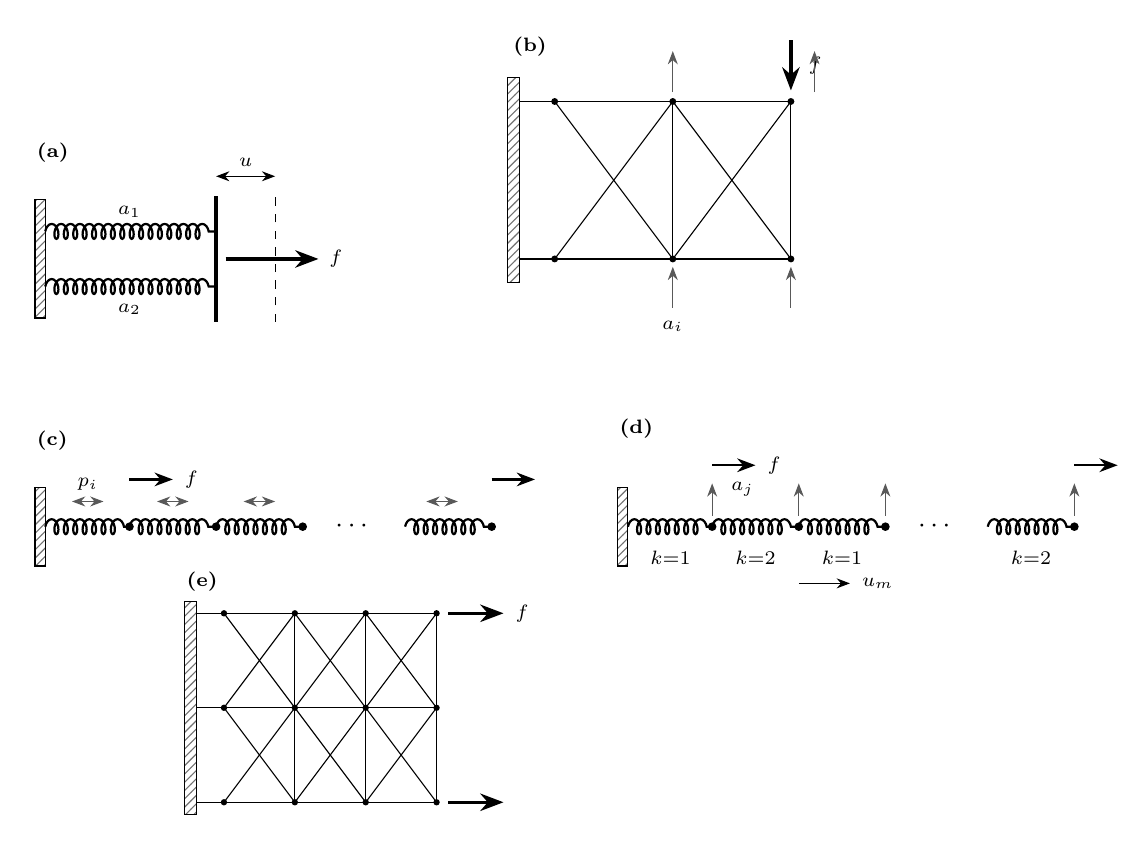
\begin{tikzpicture}[>=Stealth]
\tikzset{
  wall/.style={pattern=north east lines, pattern color=black!55},
  spr/.style={decorate, decoration={coil, aspect=0.55, segment length=3.4pt, amplitude=2.7pt}, thick},
  nd/.style={circle, fill, inner sep=1.1pt},
  act/.style={->, thin, black!65},
  mem/.style={thin}
}
% ---------- (a) two-spring demonstrator ----------
\begin{scope}
  \draw[wall] (0,-0.75) rectangle (0.13,0.75);
  \draw[spr] (0.13,0.35) -- (2.3,0.35);
  \draw[spr] (0.13,-0.35) -- (2.3,-0.35);
  \node at (1.2,0.6) {\scriptsize $a_1$};
  \node at (1.2,-0.64) {\scriptsize $a_2$};
  \draw[very thick] (2.3,-0.8) -- (2.3,0.8);
  \draw[dashed] (3.05,-0.8) -- (3.05,0.8);
  \draw[<->] (2.3,1.05) -- (3.05,1.05) node[midway,above] {\scriptsize $u$};
  \draw[->,very thick] (2.42,0) -- (3.6,0) node[right] {\scriptsize $f$};
  \node[anchor=south west] at (-0.1,1.1) {\scriptsize\bfseries (a)};
\end{scope}
% ---------- (b) ten-bar cantilever ----------
\begin{scope}[shift={(6.6,0)}]
  \draw[wall] (-0.6,-0.3) rectangle (-0.45,2.3);
  \draw[thin] (-0.45,0) -- (0,0);
  \draw[thin] (-0.45,2) -- (0,2);
  \draw[mem] (0,2) -- (1.5,2) -- (3,2);
  \draw[mem] (0,0) -- (1.5,0) -- (3,0);
  \draw[mem] (1.5,2) -- (1.5,0);
  \draw[mem] (3,2) -- (3,0);
  \draw[mem] (0,2) -- (1.5,0);
  \draw[mem] (0,0) -- (1.5,2);
  \draw[mem] (1.5,2) -- (3,0);
  \draw[mem] (1.5,0) -- (3,2);
  \foreach \p in {(0,2),(0,0),(1.5,2),(1.5,0),(3,2),(3,0)}
    \fill \p circle (1.25pt);
  \draw[->,very thick] (3,2.78) -- (3,2.14);
  \node[right] at (3.1,2.45) {\scriptsize $f$};
  \draw[act] (1.5,-0.62) -- (1.5,-0.1);
  \node[below] at (1.5,-0.66) {\scriptsize $a_i$};
  \draw[act] (3,-0.62) -- (3,-0.1);
  \draw[act] (1.5,2.12) -- (1.5,2.64);
  \draw[act] (3.3,2.12) -- (3.3,2.64);
  \node[anchor=south west] at (-0.65,2.45) {\scriptsize\bfseries (b)};
\end{scope}
% ---------- (c) chain-pretension ----------
\begin{scope}[shift={(0,-3.4)}]
  \draw[wall] (0,-0.5) rectangle (0.13,0.5);
  \draw[spr] (0.13,0) -- (1.2,0);
  \node[nd] at (1.2,0) {};
  \draw[spr] (1.2,0) -- (2.3,0);
  \node[nd] at (2.3,0) {};
  \draw[spr] (2.3,0) -- (3.4,0);
  \node[nd] at (3.4,0) {};
  \node at (4.05,0) {$\cdots$};
  \draw[spr] (4.7,0) -- (5.8,0);
  \node[nd] at (5.8,0) {};
  \draw[<->,thin,black!65] (0.47,0.32) -- (0.87,0.32);
  \node[above] at (0.67,0.34) {\scriptsize $p_i$};
  \draw[<->,thin,black!65] (1.55,0.32) -- (1.95,0.32);
  \draw[<->,thin,black!65] (2.65,0.32) -- (3.05,0.32);
  \draw[<->,thin,black!65] (4.97,0.32) -- (5.37,0.32);
  \draw[->,thick] (1.2,0.6) -- (1.75,0.6);
  \node[right] at (1.78,0.6) {\scriptsize $f$};
  \draw[->,thick] (5.8,0.6) -- (6.35,0.6);
  \node[anchor=south west] at (-0.1,0.85) {\scriptsize\bfseries (c)};
\end{scope}
% ---------- (d) dense-chain ----------
\begin{scope}[shift={(7.4,-3.4)}]
  \draw[wall] (0,-0.5) rectangle (0.13,0.5);
  \draw[spr] (0.13,0) -- (1.2,0);
  \node[nd] at (1.2,0) {};
  \draw[spr] (1.2,0) -- (2.3,0);
  \node[nd] at (2.3,0) {};
  \draw[spr] (2.3,0) -- (3.4,0);
  \node[nd] at (3.4,0) {};
  \node at (4.05,0) {$\cdots$};
  \draw[spr] (4.7,0) -- (5.8,0);
  \node[nd] at (5.8,0) {};
  \node at (0.67,-0.4) {\scriptsize $k{=}1$};
  \node at (1.75,-0.4) {\scriptsize $k{=}2$};
  \node at (2.85,-0.4) {\scriptsize $k{=}1$};
  \node at (5.25,-0.4) {\scriptsize $k{=}2$};
  \draw[act] (1.2,0.14) -- (1.2,0.55);
  \draw[act] (2.3,0.14) -- (2.3,0.55);
  \draw[act] (3.4,0.14) -- (3.4,0.55);
  \draw[act] (5.8,0.14) -- (5.8,0.55);
  \node[right] at (1.32,0.48) {\scriptsize $a_j$};
  \draw[->,thick] (1.2,0.78) -- (1.75,0.78);
  \node[right] at (1.78,0.78) {\scriptsize $f$};
  \draw[->,thick] (5.8,0.78) -- (6.35,0.78);
  \draw[->] (2.3,-0.72) -- (2.95,-0.72);
  \node[right] at (2.98,-0.72) {\scriptsize $u_m$};
  \node[anchor=south west] at (-0.1,1.0) {\scriptsize\bfseries (d)};
\end{scope}
% ---------- (e) cross-braced lattice ----------
\begin{scope}[shift={(2.4,-6.9)}]
  \draw[wall] (-0.5,-0.15) rectangle (-0.35,2.55);
  \draw[thin] (-0.35,0) -- (0,0);
  \draw[thin] (-0.35,1.2) -- (0,1.2);
  \draw[thin] (-0.35,2.4) -- (0,2.4);
  \draw[mem] (0,0) -- (2.7,0);
  \draw[mem] (0,1.2) -- (2.7,1.2);
  \draw[mem] (0,2.4) -- (2.7,2.4);
  \foreach \j in {1,2,3} \draw[mem] (0.9*\j,0) -- (0.9*\j,2.4);
  \foreach \j in {0,1,2} {
     \draw[mem] (0.9*\j,0) -- (0.9*\j+0.9,1.2);
     \draw[mem] (0.9*\j,1.2) -- (0.9*\j+0.9,0);
     \draw[mem] (0.9*\j,1.2) -- (0.9*\j+0.9,2.4);
     \draw[mem] (0.9*\j,2.4) -- (0.9*\j+0.9,1.2);
  }
  \foreach \j in {0,1,2,3} \foreach \i in {0,1,2}
     \fill (0.9*\j,1.2*\i) circle (1.15pt);
  \draw[->,very thick] (2.85,2.4) -- (3.55,2.4);
  \node[right] at (3.58,2.4) {\scriptsize $f$};
  \draw[->,very thick] (2.85,0) -- (3.55,0);
  \node[anchor=south west] at (-0.6,2.55) {\scriptsize\bfseries (e)};
\end{scope}
\end{tikzpicture}
\captionof{figure}{Schematic of the demonstrator and the four benchmark
families, drawn after the artifact's model generators (not to scale).
(a)~Two-spring demonstrator of Section~\ref{sec:two-spring}: two unit
springs in parallel anchor a rigid bar to the wall; the load \(f\) and
the two actuator commands \(a_1,a_2\) determine the bar displacement
\(u=(f-a_1-a_2)/2\) (displaced position dashed).
(b)~Ten-bar family: the classic six-node cantilever with two \(3\times4\)
bays and \(3\)--\(4\)--\(5\) diagonals; grey arrows mark the four
vertical node-force actuators at the free nodes, the black arrow the
quantised tip loads, and member forces are monitored.
(c)~Chain-pretension family: unit springs grounded at one end, each
carrying a self-equilibrated pre-tension pair (double arrows, \(p_i\));
spring forces are monitored and the two load scenarios act at the chain
ends.
(d)~Dense-chain family: alternating spring stiffnesses \(1\) and \(2\),
one node-force actuator per node (grey arrows), a monitored mid-chain
displacement \(u_m\), and end loads.
(e)~Lattice family: the cross-braced lattice with two bay-rows and \(C\)
columns (three shown), fully supported at the left edge; pre-tension
pairs act on the verticals and diagonals, member forces are monitored,
and the two quantised loads act at the free-edge corners.
Table~\ref{tab:mechanics-families} records the corresponding influence
structure and widths.}
\label{fig:mechanics-families}
\end{center}

Table~\ref{tab:mechanics-benchmarks} reports the recorded gate: all twenty
row batches are independently verified, all eighteen constructed
decompositions are validated, all eighteen dynamic-programming certificates
are re-verified, each constructed split instance is solved with a verified
optimum policy and each constructed same instance is refuted with a verified
\texttt{DP-REFUTATION}, while the two remaining cases, the largest lattice
instances, carry certified influence scopes and recorded scope widths but no
constructible instance: their relation tables exceed the enumeration cap and
are marked
\texttt{RELATION-TABLE-LIMIT}.  Corrupted row batches and
corrupted dynamic-programming certificates are rejected on the small
representatives.  The ten-bar family is cross-validated against the exact
affine row generator of Section~\ref{sec:mechanics-front-end}: the derived
finite instances agree.  Its same-observation instance carries a brute-force
sensor-repair certificate selecting one threshold sensor with certified
optimality, so the quantised-sensor structure of the two-spring demonstrator
reappears in a structural model.

\begin{center}
\footnotesize
\setlength{\tabcolsep}{4pt}
\begin{tabular}{@{}lrrrrrr@{}}
\toprule
Instance & \(\lvert X\rvert\) & rows & width & status & DP (s) & verify (s)\\
\midrule
ten-bar, same & 4 & 20 & 3 & \texttt{UNSAT} & 0.001 & 0.001\\
ten-bar, split & 8 & 20 & 3 & \texttt{OPT} & 0.001 & 0.001\\
chain \(n{=}8\), same / split & 8 / 16 & 16 & 0 & \texttt{UNSAT} / \texttt{OPT} & 0.000 / 0.001 & 0.000 / 0.001\\
chain \(n{=}256\), same / split & 256 / 512 & 512 & 0 & \texttt{UNSAT} / \texttt{OPT} & 0.011 / 0.031 & 0.018 / 0.059\\
chain \(n{=}1024\), same / split & 1024 / 2048 & 2048 & 0 & \texttt{UNSAT} / \texttt{OPT} & 0.097 / 0.292 & 0.159 / 0.548\\
dense-chain \(n{=}8\), same / split & 8 / 16 & 2 & 7 & \texttt{UNSAT} / \texttt{OPT} & 0.006 / 0.012 & 0.009 / 0.017\\
dense-chain \(n{=}16\), same / split & 16 / 32 & 2 & 15 & \texttt{UNSAT} / \texttt{OPT} & 2.37 / 4.57 & 3.06 / 6.33\\
lattice \(C{=}1\), same / split & 6 / 12 & 18 & 5 & \texttt{UNSAT} / \texttt{OPT} & 0.002 / 0.003 & 0.002 / 0.004\\
lattice \(C{=}2\), same / split & 12 / 24 & 36 & 11 & \texttt{UNSAT} / \texttt{OPT} & 0.138 / 0.307 & 0.217 / 0.328\\
lattice \(C{=}3\), scopes & --- & 54 & 17 & \texttt{RELATION-TABLE-LIMIT} & --- & ---\\
lattice \(C{=}4\), scopes & --- & 72 & 23 & \texttt{RELATION-TABLE-LIMIT} & --- & ---\\
\bottomrule
\end{tabular}
\captionof{table}{Recorded mechanics benchmark gate (selected sizes;
the artifact's recorded reports contain all twenty cases and timings).  Every constructed
same-observation instance is refuted with a verified certificate and every
constructed split instance
solved with a verified optimum policy, including the 1024-spring chain and
the width-11 lattice.  Status entries abbreviate the four-status discipline
of Remark~\ref{rem:status-discipline}: \texttt{UNSAT} and \texttt{OPT}
record verified \texttt{DP-REFUTATION} and \texttt{DP-OPTIMUM} certificates,
that is, \texttt{CERTIFIED-UNSAT} and \texttt{CERTIFIED-OPT}.  Lattice column
counts three and four have certified
influence scopes but relation tables beyond the enumeration
limit (\texttt{RELATION-TABLE-LIMIT}), so no instance is constructed for
them; for these two rows the artifact's recorded width field is the
influence-scope size (18 and 24 actuators --- every certified row's scope is
the full actuator set, so the primal graph is complete), and the tabulated
17 and 23 are the treewidths this forces, continuing the \(6C-1\) growth of
the constructed lattices.}
\label{tab:mechanics-benchmarks}
\end{center}

Three recorded observations carry structural content.  First, the
pre-tensioned chain certifies refutations at 1024 springs with width-0
decompositions: the exact locality of self-equilibrated pre-tension makes
the finite presentation bounded-width at every scale, and the pipeline cost
is dominated by certified relation generation rather than by search.  Second,
the dense-influence families realise the width boundary: the measured scope
of every row equals the full actuator set, so decomposition width grows
linearly and the relation tables themselves exceed the enumeration limit at
moderate sizes.  Third, the sensor structure is decisive at every scale: the
same-observation instances are unsatisfiable and the split instances
satisfiable in every recorded family case, with the ten-bar repair
certificate recorded above exhibiting
the minimal separating sensor.

\section{Width-adaptive sparsification study}
\label{sec:sparsification-study}

The sparsification ladder of Section~\ref{sec:sparsification} is evaluated
on retained-scope ladders by structural proximity: the retained scope of a
row at radius \(r\) keeps the actuators anchored within member-graph
distance \(r\) of the monitored member or node, and the full radius is the
no-sparsification ablation.  For every rung the study verifies the
sparsification certificate and the pairwise ladder monotonicity with the
previous rung, solves the inner and outer instances with verified
dynamic-programming certificates, and classifies the bracket through the rows
of Table~\ref{tab:ladder-outcomes}: certified
satisfiable when an inner policy, extended by zeros on the omitted
actuators (every completion of an inner-retained assignment is certified
safe, so the zero completion is one), verifies exactly against the full
certified rows; certified
unsatisfiable when the outer model is refuted, which is sound because outer
relations contain the true relations; and inconclusive when the inner model
is unsatisfiable while the outer model is satisfiable.  Both observation
variants are evaluated at every rung.

\begin{center}
\begin{tabular}{@{}llrrrl@{}}
\toprule
Family & radius & retained & inner width & unresolved & brackets (same / split)\\
\midrule
ten-bar & 0 & 1.6 & 3 & 0.50 & inconclusive / inconclusive\\
ten-bar & 1--full & 4.0 & 3 & 0.00 & certified / certified\\
chain \(n{=}64\) & 0--full & 1.0 & 0 & 0.00 & certified / certified\\
dense-chain \(n{=}12\) & 0 & 1.0 & 0 & 1.00 & inconclusive / inconclusive\\
dense-chain \(n{=}12\) & 1 & 3.0 & 2 & 1.00 & inconclusive / inconclusive\\
dense-chain \(n{=}12\) & 2 & 5.0 & 4 & 1.00 & inconclusive / inconclusive\\
dense-chain \(n{=}12\) & 3 & 7.0 & 6 & 1.00 & inconclusive / inconclusive\\
dense-chain \(n{=}12\) & full & 12.0 & 11 & 0.00 & certified / certified\\
lattice \(C{=}1\) & 0 & 0.67 & 0 & 0.33 & inconclusive / inconclusive\\
lattice \(C{=}1\) & 1 & 3.56 & 5 & 0.15 & inconclusive / inconclusive\\
lattice \(C{=}1\) & 2--full & 5.56 & 5 & 0.00 & certified / certified\\
lattice \(C{=}2\) & 0 & 0.67 & 0 & 0.64 & inconclusive / inconclusive\\
lattice \(C{=}2\) & 1 & 6.0 & 11 & 0.27 & inconclusive / inconclusive\\
lattice \(C{=}2\) & full & 12.0 & 11 & 0.00 & certified / certified\\
lattice \(C{=}3\) & 0 & 0.67 & 0 & 0.70 & inconclusive / inconclusive\\
lattice \(C{=}3\) & 1 & 6.67 & 14 & 0.34 & inconclusive / inconclusive\\
\bottomrule
\end{tabular}
\captionof{table}{Recorded width-adaptive sparsification study (selected
rungs; the artifact's recorded reports contain the complete ladder data).  Retained
is the mean retained-scope size; unresolved is the mean share of outer rows
that are not inner rows; brackets are the certified or inconclusive
classifications of the same- and split-observation variants.  The complete
study covers twenty rungs --- a ten-bar ladder of four radii, a two-rung
chain-pretension ablation whose rungs coincide because radius 0 already
retains every scope (displayed as the single range \(0\)--full), a dense-chain ladder of five radii, and lattice
ladders of four, three, and two radii at column counts one, two, and three
--- with fourteen
verified ladder steps; the compressed radius ranges mark consecutive rungs
whose brackets certify, and the recorded values shown are those of the
finest rung of each range, whose inner widths agree with the full-instance
widths of Table~\ref{tab:mechanics-benchmarks}.  All 20
sparsification certificates and 14 ladder steps verify; the dense instance
of lattice \(C{=}3\) is beyond the relation-table enumeration limit
(\texttt{RELATION-TABLE-LIMIT}).}
\label{tab:sparsification-study}
\end{center}

The recorded outcome of Table~\ref{tab:sparsification-study} is a soundness result with an honest negative
component.  Monotonicity holds and is certified at every ladder step, the
unresolved fraction decreases monotonically with the radius in every family,
and the brackets agree with the true statuses at the full radius.  But on
the calibrated families the brackets certify only at or near the full
radius: the omitted-interval tails dominate the declared safety windows at
small radii, so aggressive sparsification is sound yet inconclusive, and the
retained scopes at intermediate radii overlap enough that the inner width
need not drop below the dense width.  The study therefore supports the
ladder theorem and the bracket discipline, and records that the calibrated
models do not yet exhibit a practical width-reduction benefit from
proximity-based retention.

\section{Prototype artifact and reproducibility}
\label{sec:artifact}

The artifact includes explicit-table solving, tree-decomposition DP
certificates, exact affine row certificates, sparsification certificates,
controlled-width benchmark generation, baseline encoders for DIMACS CNF,
LP-format MILP, and a minimal CP-SAT representation, optional
external-solver adapters, a fixed-hardware external-baseline sweep,
external-result cross-checking, report summaries, and SVG plot generation.
The mechanics layer adds an exact rational structural front end with
independently verified row batches, the four benchmark families with both
observation variants, minimum-fill decompositions, the sparsification ladder
study, and the comparative scaling study on mechanics-derived instances,
together with its version-exact replication and dense-family extension
drivers and the forensic audit tools for the recorded reports.
The repository-ready entry point is
\begin{verbatim}
make reproduce
\end{verbatim}
with \texttt{./reproduce.sh} as an equivalent shell command.
Appendix~\ref{app:artifact} documents the certificate formats and the
reproduction and archive protocols in detail.

A compact verification table from the verification gate is as follows; the
phase labels follow the artifact's recorded build phases, phase~6 being the
recorded mechanics comparative-scaling study.
\begin{center}
\begin{tabular}{@{}p{0.58\linewidth}p{0.28\linewidth}@{}}
\toprule
Gate & Status\\
\midrule
Two-spring, same observation & \texttt{CERTIFIED-UNSAT}\\
Two-spring, split observation & \texttt{CERTIFIED-SAT}\\
Fibre conflict certificate & \texttt{VERIFIED}\\
Corrupted fibre certificate & \texttt{REJECTED}\\
Threshold sensor repair & \texttt{CERTIFIED-OPT}\\
Tree-decomposition optimum certificate & \texttt{VERIFIED}\\
Tree-decomposition refutation certificate & \texttt{VERIFIED}\\
Exact affine \texttt{FE-ROW} batch & \texttt{VERIFIED}\\
Corrupted \texttt{FE-ROW} batch & \texttt{REJECTED}\\
Sparsification ladder & \texttt{VERIFIED}\\
External baseline sweep, five solvers & \texttt{COMPLETE}\\
External satisfiable-model cross-checks & \texttt{VERIFIED}\\
External refutation cross-checks & \texttt{VERIFIED}\\
Mechanics row batches, twenty cases & \texttt{VERIFIED}\\
Corrupted mechanics row batch & \texttt{REJECTED}\\
Corrupted mechanics DP certificate & \texttt{REJECTED}\\
Ten-bar affine cross-validation & \texttt{VERIFIED}\\
Ten-bar threshold sensor repair & \texttt{CERTIFIED-OPT}\\
Mechanics sparsification certificates & \texttt{VERIFIED}\\
Mechanics ladder monotonicity steps & \texttt{VERIFIED}\\
Mechanics baseline sweep, five solvers & \texttt{COMPLETE}\\
Phase-6 sweep replication, five solvers & \texttt{COMPLETE}\\
Dense-extension generation, four cases & \texttt{VERIFIED}\\
Dense-extension DP memory-limit case & \texttt{INCONCLUSIVE}\\
Dense-extension sweep, five solvers & \texttt{COMPLETE}\\
Dense-extension external cross-checks & \texttt{VERIFIED}\\
Recorded sweep counters vs per-instance records & \texttt{VERIFIED}\\
\bottomrule
\end{tabular}
\captionof{table}{Recorded verification-gate rows (selected).  The
mathematical statuses follow the four-status discipline of
Remark~\ref{rem:status-discipline}: \texttt{CERTIFIED-SAT},
\texttt{CERTIFIED-UNSAT}, and \texttt{CERTIFIED-OPT} transport certified
claims, and \texttt{INCONCLUSIVE} records the absence of one.
\texttt{VERIFIED}, \texttt{REJECTED}, and \texttt{COMPLETE} are bookkeeping
markers for the state of a gate check, not answers.}
\label{tab:verification-gate}
\end{center}

Controlled-width benchmark families include paths, binary trees,
banded chains, and small grids with supplied decompositions, together with an
unsatisfiable odd-ring family carrying a supplied path decomposition of width
two.  The reports record instance size, ordinary width, weighted width,
certificate size, and verification time.  These are certificate and
reproducibility checks; the external-baseline comparison below reports measured
timings under a fixed configuration without asserting an advantage of the
native pipeline.

\subsection{External baseline comparison on identical instances}
\label{subsec:external-baselines}

A fixed-hardware external-baseline experiment compares the native pipeline with
five external solvers on identical finite instances.  The recorded
configuration is: a two-core Intel Xeon virtual machine with 4.1\,GiB of
memory, Debian GNU/Linux 13 with kernel 5.10.134 and glibc 2.41, and
harness Python 3.12.14; minisat (2.2 series, built from the public mirror at commit
16982a5 with gcc 14.2 at optimisation level \texttt{-O3} and the standard
compiler-compatibility patch), kissat 4.0.4 (commit 8af8e56, gcc 14.2,
\texttt{-O3}), z3 5.1.0, CP-SAT
from OR-Tools 9.15.6755, and HiGHS 1.15.1; a 60-second wall-clock timeout,
enforced as a hard kill at sixty seconds for the subprocess SAT solvers and,
for the in-process CP-SAT and HiGHS runners and the bounded native runner, at
ninety seconds, the thirty-second grace covering interpreter startup and model
construction; a
3\,GiB address-space cap; three repetitions per solver and instance with the
median reported; single-threaded deterministic configurations throughout, with
CP-SAT restricted to one worker and a fixed random seed.  The artifact's
protocol block machine-records the processor, core count, memory, kernel
version, glibc version, and harness Python; the distribution name, Debian
GNU/Linux 13, is stated from the operator's environment record rather than
machine-captured, and is consistent with the recorded glibc 2.41 userland.
Timings are whole-process wall clock and include solver startup; the CP-SAT and HiGHS
timings additionally include interpreter startup and model construction.

Every instance is generated as a finite ECD presentation and encoded once by
the artifact's encoders, so that all solvers receive the same finite relation
data: DIMACS CNF for minisat, kissat, and z3; the LP-format MILP encoding for
HiGHS; and the minimal forbidden-tuple encoding for CP-SAT.  The families are
the controlled-width benchmark families (path disequality chains, binary
trees, banded chains at width two, and two-row grids) and the unsatisfiable
odd-ring family; instance sizes range from 5 to 2048 policy variables.  On each
instance the native tree-decomposition dynamic program is run with the supplied
decomposition and timed, its certificate is independently re-verified and
timed, and for satisfiable instances a policy is reconstructed from the
certificate and verified.  The experiment covers 24 instances and 120 external
solver runs.

Table~\ref{tab:external-baselines} reports median wall-clock times at the
largest instance of each family; the artifact report contains the full
per-instance data, including minimum and maximum repetitions and peak memory.

\begin{center}
\begin{tabular}{@{}lrrrrrrrrr@{}}
\toprule
Family & $|X|$ & clauses & DP & verify & minisat & kissat & z3 & CP-SAT & HiGHS\\
\midrule
path-neq & 2048 & 4094 & 0.388 & 0.682 & 0.006 & 0.004 & 0.007 & 0.611 & 0.130\\
binary-tree-neq & 1023 & 2044 & 0.135 & 0.211 & 0.004 & 0.003 & 0.005 & 0.382 & 0.122\\
banded-chain-w2 & 2048 & 4092 & 0.546 & 0.930 & 0.006 & 0.004 & 0.008 & 0.418 & 0.284\\
grid-neq $2\times 256$ & 512 & 1532 & 0.055 & 0.087 & 0.004 & 0.003 & 0.004 & 0.370 & 0.116\\
odd-ring-neq & 1025 & 2050 & 0.169 & 0.304 & 0.005 & 0.003 & 0.005 & 0.371 & 0.121\\
\bottomrule
\end{tabular}
\captionof{table}{Median whole-process wall-clock times in seconds at the
largest instance of each family, as recorded in
\texttt{reports/external\_baseline\_sweep.json}.  DP and verify are the native dynamic program
and its independent certificate re-verification; the odd-ring family is
unsatisfiable, the others satisfiable.}
\label{tab:external-baselines}
\end{center}

The cross-check accounting is complete: all 120 external runs agree with the
native certificates; each of the 95 external satisfiable models is parsed,
converted to a policy on the original instance, and verified natively; each of
the 25 external unsatisfiable answers is checked against an independently
verified \texttt{DP-REFUTATION} certificate; no run is inconclusive or
rejected.  Peak resident memory of any external run is at most 100.2\,MiB
against the 3\,GiB cap.  At these certificate-study sizes the
compiled SAT solvers complete in milliseconds, with startup dominating the
measurement, while the reference native implementation is a Python program
whose wall-clock cost is dominated by certificate emission and independent
verification rather than search.  The experiment therefore supports the
reproducibility and cross-checking claims of this article; it does not support,
and the article does not make, a performance-superiority claim over the
external solvers.

\subsection{Comparative scaling study on mechanics instances}
\label{subsec:mechanics-baselines}

The fixed external-baseline protocol is applied unchanged to fourteen
Boolean instances derived from the mechanics families: both observation
variants of the ten-bar truss, the pre-tensioned chain at 256 and 1024
springs, the dense-influence chain at 8 and 16 actuators, and the lattice at
one and two columns.  Identical encodings are emitted once; every external
run is bounded by the 60-second timeout, the 3\,GiB address-space cap, and
the single-threaded deterministic configurations; timings are medians of
three repetitions.  The native pipeline runs as a bounded isolated process
that loads the instance, runs the dynamic program, re-verifies its
certificate, and reconstructs and verifies a policy when satisfiable, so
native and external wall-clock figures cover comparable whole-process
pipelines.  Certified relation generation and its independent verification
are accounted separately from the recorded mechanics benchmark suite and
excluded from both sides.

\begin{center}
\footnotesize
\begin{tabular}{@{}lrrrrrrrr@{}}
\toprule
Instance & \(\lvert X\rvert\) & clauses & native & mini. & kissat & z3 & CP-SAT & HiGHS\\
\midrule
ten-bar, same & 4 & 82 & 0.07 & 0.003 & 0.002 & 0.003 & 0.363 & 0.106\\
ten-bar, split & 8 & 82 & 0.12 & 0.003 & 0.002 & 0.012 & 0.384 & 0.127\\
chain \(n{=}256\), same & 256 & 512 & 0.12 & 0.005 & 0.002 & 0.004 & 0.388 & 0.122\\
chain \(n{=}1024\), same & 1024 & 2048 & 0.37 & 0.003 & 0.002 & 0.004 & 0.366 & 0.115\\
chain \(n{=}1024\), split & 2048 & 2048 & 1.02 & 0.003 & 0.002 & 0.005 & 0.370 & 0.116\\
dense \(n{=}8\), same & 8 & 487 & 0.12 & 0.004 & 0.002 & 0.003 & 0.358 & 0.112\\
dense \(n{=}16\), same & 16 & 130942 & 7.18 & \texttt{TMO} & 3.775 & 1.648 & 49.5 & \texttt{TMO}\\
dense \(n{=}16\), split & 32 & 130942 & 14.54 & \texttt{TMO} & 0.367 & 0.355 & 4.289 & 5.203\\
lattice \(C{=}1\), same & 6 & 196 & 0.12 & 0.003 & 0.002 & 0.003 & 0.372 & 0.115\\
lattice \(C{=}2\), same & 12 & 26568 & 0.92 & 2.002 & 0.139 & 0.474 & 1.716 & 6.034\\
lattice \(C{=}2\), split & 24 & 26568 & 1.47 & 1.294 & 0.034 & 0.569 & 0.860 & 0.946\\
\bottomrule
\end{tabular}
\captionof{table}{Median whole-process wall-clock times in seconds for the
comparative scaling study on mechanics-derived instances (selected cases;
the artifact report contains all fourteen).  \texttt{TMO} marks runs that
exceeded the fixed 60-second limit and are recorded as inconclusive.  Native
timings cover the whole bounded pipeline including certificate emission and
independent re-verification.  The recorded study was replicated in full under
version-exact solver provenance with an identical summary; see
Subsection~\ref{subsubsec:replication-extension}.}
\label{tab:mechanics-baselines}
\end{center}

The cross-check accounting over the runs of
Table~\ref{tab:mechanics-baselines} is complete: all fourteen native certificates
verify; 34 external satisfiable models are verified natively as policies;
33 external unsatisfiable answers are cross-checked against verified
\texttt{DP-REFUTATION} certificates; three external runs exceed the limit
and are recorded as inconclusive; nothing is rejected; and all 67 status-bearing
external answers agree with the native
certificates.\footnote{A forensic audit of the recorded artifact confirms the
recorded counters against the per-instance records: the CP-SAT run on the
unsatisfiable dense \(n{=}16\) instance answered \texttt{UNSAT} in 49.5\,s
with a verified cross-check, not \texttt{UNKNOWN}; a version-exact
replication reproduces the same answer and the same summary; and the
runner code maps a CP-SAT \texttt{UNKNOWN} status to inconclusive by
construction, so it cannot be bucketed with unsatisfiable answers.  The
harness agreement counter is gated on verified cross-check evidence,
which makes the accounting identity structural.  An earlier version of
this article reported a ``corrected'' accounting of 32 cross-checked
unsatisfiable answers, 4 inconclusive runs, and 66 agreements, on the
mistaken belief that the CP-SAT run had returned \texttt{UNKNOWN}; that
correction is itself withdrawn.}
Finite-element (FE) preprocessing for the dense instances amounts to about 2.7 seconds of
certified relation generation and 2.7 seconds of verification, reported
separately.

The recorded observations are per-instance and carry no superiority claim.
On the width-bounded families every solver answers in milliseconds and the
native Python pipeline is slower in wall-clock, consistent with the earlier
external-baseline experiment.  On the dense-influence family at sixteen
actuators, whose forbidden-tuple encoding has 130{,}942 clauses, minisat
exceeds the limit on both observation variants and HiGHS exceeds it on the
unsatisfiable variant, while kissat answers in 3.8 seconds, z3 in 1.7
seconds, CP-SAT certifies the unsatisfiable variant in about 50 seconds,
and the native dynamic program certifies the refutation in 7.2 seconds of
wall-clock including certificate emission and verification.  The
native certificates on this family grow as \(2^{n}\) (57 and 116\,MB at
\(n{=}16\), and 120, 243, and 253\,MB at \(n{=}17\) and \(n{=}18\) in
the extension below), which is the recorded cost of the certificate-emitting
pipeline and the honest boundary of the dense family in this artifact.

\subsubsection{Version-exact replication and dense-family extension}
\label{subsubsec:replication-extension}

Two follow-up studies of the artifact release consolidate the recorded comparative
scaling study: a full replication under version-exact solver provenance,
and an extension of the dense-influence family beyond the recorded boundary
\(n{=}16\).

\paragraph{Full replication.}
The complete fourteen-instance sweep was re-executed with all five solvers
rebuilt or pinned to the recorded versions of
Subsection~\ref{subsec:external-baselines}.
The replication reproduces the recorded summary exactly --- fourteen
verified native certificates, 34 verified satisfiable cross-checks, 33
verified unsatisfiable cross-checks, three inconclusive runs, and 67
agreements --- and a field-by-field comparison
(\texttt{diff\_reports.py}, timing and size fields excluded as
hardware-dependent) finds 1135 matching leaf fields whose only mismatches are
the certificate file names, the per-case provenance notes carried only by the
recorded report, and the hardware block's memory figure (3.9 against
4.1\,GiB); the replication's native runner re-emits byte-identical duplicate
certificates, with SHA-256 equality verified for the dense-8 and dense-16
same, ten-bar same, and lattice \(C{=}2\) split certificates and for the
three completed dense-17/18 certificates of the extension below.
The replicated report is archived in \texttt{reports/} as
\texttt{mechanics\_external\_baseline\_sweep\_v2.json}.

\paragraph{Dense-family extension.}
The dense-influence family is extended to \(n{=}17\) and \(n{=}18\), both
observation variants, with the recorded phase-4 driver (the
mechanics-benchmark generator) and the fixed
protocol unchanged.  Generation certifies all four FE row batches and
tree decompositions (widths 16, 16, 17, and 17); the dynamic program
certifies a refutation at \(n{=}17\) same (120.2\,MB certificate), an
optimum with a verified policy at \(n{=}17\) split (243.2\,MB), and a
refutation at \(n{=}18\) same (252.5\,MB); at \(n{=}18\) split the
certificate-emitting dynamic program exceeds the machine's physical memory
during message construction --- the generating process was killed by the
kernel out-of-memory (OOM) killer with an anonymous resident set of 3\,750\,608\,kB, about
3.6\,GiB, the kernel line being retained with the failure record --- and the
case is recorded
as \texttt{DP-MEMORY-LIMIT} with its model, certified row batch, instance,
and validated decomposition archived.  The comparative sweep then applies
the fixed external-baseline protocol unchanged to the four extension
instances.

\begin{center}
\footnotesize
\begin{tabular}{@{}lrrrrrrr@{}}
\toprule
Instance & clauses & native & mini. & kissat & z3 & CP-SAT & HiGHS\\
\midrule
dense \(n{=}17\), same & 262002 & 15.2 & \texttt{TMO} & 15.95 & 4.90 & \texttt{UNK} & \texttt{TMO}\\
dense \(n{=}17\), split & 262002 & 30.9 & \texttt{TMO} & 0.81 & 0.75 & 8.81 & 13.02\\
dense \(n{=}18\), same & 524123 & 31.6 & \texttt{TMO} & 52.18 & \texttt{TMO} & \texttt{TMO} & \texttt{TMO}\\
dense \(n{=}18\), split & 524123 & \texttt{MEM} & \texttt{TMO} & 3.30 & 1.71 & \texttt{UNK} & 29.89\\
\bottomrule
\end{tabular}
\captionof{table}{Median whole-process wall-clock times in seconds for the
dense-family extension at \(n{=}17\) and \(n{=}18\).  Native timings cover
the whole bounded pipeline including certificate emission and independent
re-verification; \texttt{TMO} marks runs that ended at or beyond the
wall-clock limits without a recognised status; \texttt{UNK} marks CP-SAT
runs that returned \texttt{UNKNOWN}; \texttt{MEM} marks the bounded native
run that raised \texttt{MemoryError} at the 3\,GiB address-space cap; all
marked runs are recorded as inconclusive.  The limits are two-tier as in the
recorded study: the in-process CP-SAT and HiGHS runners carry a sixty-second
solver limit with a ninety-second hard process cap whose grace covers
interpreter startup and model construction.  Every status-bearing external answer is
cross-checked: unsatisfiable answers against the verified
\texttt{DP-REFUTATION} certificates of the same cases, satisfiable models
as natively verified policies.}
\label{tab:dense-extension}
\end{center}

As in the recorded study, the observations are per-instance and carry no
superiority claim.  minisat exceeds the limit on all four extension instances; CP-SAT ends
without a recognised status on the three unsatisfiable or encoding-heaviest
variants, whose forbidden-tuple encodings comprise 137.7--388.1\,MB of JSON:
it returns \texttt{UNKNOWN} within its solver limit on the \(n{=}17\) same
variant (40\,s), overshoots the soft sixty-second solver limit before
returning \texttt{UNKNOWN} on the \(n{=}18\) split variant (73\,s of solve
time), and is killed at the ninety-second hard process cap on the
\(n{=}18\) same variant;
kissat and z3 answer both \(n{=}17\) variants in seconds; kissat is the
only solver answering the unsatisfiable \(n{=}18\) variant within the limit
(52.2\,s); and on the satisfiable \(n{=}18\) split variant kissat, z3, and
HiGHS return models that verify natively as policies while the
certificate-emitting native pipeline cannot complete within the same
3\,GiB address-space cap.  The cross-check accounting over the twenty
extension runs of Table~\ref{tab:dense-extension} records seven verified
satisfiable models, three verified unsatisfiable answers, ten inconclusive
runs, no rejections, and seven
agreements with the native certificates --- the three verified
satisfiable answers at \(n{=}18\) split have no native status to agree
with, since the native run is inconclusive at the memory cap.  FE
preprocessing is accounted separately as in the recorded study, and the
extension reports
(\texttt{mechanics\_dense\_extension.json}, \\
\texttt{mechanics\_dense\_extension\_sweep.json}) are archived with the
artifact.

The artifact, including the prototype, the reproduction scripts, the recorded
reports, the replication and dense-extension reports of
Subsection~\ref{subsubsec:replication-extension}, and the release manifest
with the full solver build provenance, is archived in the project repository
\texttt{https://github.com/\allowbreak MIKEAA2020/\allowbreak halting-physics}
under release tag
\texttt{halting\_\allowbreak physics\_\allowbreak workspace\_\allowbreak v4}.  Extension
artifacts above the repository's per-file size limit are archived by SHA-256
checksum and size in the release manifest and are exactly regenerable from
the archived instances and decompositions; the small artifacts are deposited
with their checksums; the archive mechanics are recorded in
Appendix~\ref{app:artifact}.  An archival DOI will be assigned before
publication.

\section{Limitations and conclusions}
\label{sec:limitations}

The companion theory is deliberately finite and certificate-driven.  It does not
claim a universal dichotomy for all finite ECD instances, practical superiority
over generic solvers, or continuum-mechanics validity from finite algebraic row
certificates alone.  More specifically, it does not claim that inner-model
infeasibility proves physical infeasibility, that solver timeout proves bounded
nonrealisability, that the sparsification theorem is practically useful on every
mechanical model, or that the \(\mathsf
D^{\mathsf P}\)~\cite{papadimitriou94}, ETH~\cite{impagliazzo-paturi01},
W[1] and W[2]~\cite{downey-fellows99}
frontiers have been proved for every finite ECD layer; the W[2]-hardness of
sensor repair (Proposition~\ref{prop:sensor-design-hardness}) is the one
design-side reduction this article records, a single problem rather than a
layer.  Those statements require
additional reductions, modelling hypotheses, or experiments.  The recorded
mechanics study adds its own boundaries: the structural front end certifies
declared rational models, not discretisation error; the dense-influence families
exhaust the relation-table and certificate-size limits of the pipeline at
moderate sizes; the sparsification ladders certify monotonicity while remaining
inconclusive at reduced radii on the calibrated families; and the comparative
scaling study records per-instance observations only, in which external solvers
and the native pipeline each fail and succeed on different instances of one
family under the fixed protocol.

The positive claim is narrower and checkable: once a finite source
representation is declared, the solver and verifier can produce typed evidence
for policies, refutations, optimum costs, sensor repairs, finite mechanical
relations, and sparsification ladders.  The location of failure remains part of
the presentation, and the certificate records the data needed to transport that
claim.

\input{companion-artifact-appendix-v9.tex}

\section{Standard reductions for the explicit-table frontier}
\label{app:reductions}

This appendix records the encodings and standard reductions behind the
complexity table of Section~\ref{sec:complexity}, in the explicit-table
input format of Section~\ref{sec:finite-presentations}.  The membership
parts are immediate from the format; the reductions are standard and are
stated at the encoding level so that the verifier-facing representation is
unchanged.  All reductions satisfy the nonempty-local-relation promise: no
factor table of the constructed instance is empty.

\subsection{Tractable rows}

Verifying a proposed assignment scans the factor tables, so it is linear in
the input size.  Unary constraints filter the domains variable by variable.
Every Boolean binary factor is a conjunction of 2-clauses, one per forbidden
tuple: forbidding \((v_1,v_2)\) on \((x,y)\) is the clause
\((x\ne v_1)\lor(y\ne v_2)\).  Boolean binary instances are therefore
2-SAT formulas and are decided in linear time~\cite{apt79}.

\subsection{Hard rows}

Boolean ternary factors are NP-complete: a 3-CNF clause
\((\ell_1\lor\ell_2\lor\ell_3)\) becomes a factor on its three variables
whose table permits the seven satisfying tuples, and the satisfying
assignments of the formula are exactly the global assignments of the
instance.  Membership in NP is witnessed by the assignment.  The
fixed-template background is classified by the dichotomy
theorems~\cite{schaefer78,zhuk17}.

Binary disequality over a three-element domain is NP-complete by graph
3-colourability: vertices become variables with domain \(\{1,2,3\}\), and
edges become disequality factors whose tables permit six of nine
tuples~\cite{gareyjohnson79}.

Nonexistence of a global assignment is coNP-complete: it is the complement
of the ternary satisfiability problem above, and a satisfying assignment is
the polynomial witness for existence.

Counting global assignments is \#P-complete: the same clause-to-factor
encoding reduces \#3-SAT, and counting the satisfying assignments of the
formula is counting the global assignments of the
instance~\cite{valiant79,creignou-hermann96}.

Minimum-cardinality fibre obstruction is NP-hard from set
cover~\cite{karp72}.  Given a universe \(A\) and sets \(X_1,\dots,X_n
\subseteq A\), build one observation fibre with action set \(A\) and one
scenario \(w_j\) per set \(X_j\) with admissible set \(S_{w_j}=A\setminus
X_j\).  A set \(C\) of scenarios has empty admissible intersection if and
only if \(\bigcup_{w_j\in C}X_j=A\), so minimum-cardinality conflict cores
are exactly minimum set covers.  The local relations are nonempty whenever
\(X_j\ne A\), which holds after discarding redundant set rows.

Minimum-cardinality sensor repair from a listed candidate family is
NP-complete from set cover~\cite{karp72}.  Given a universe \(U\), covering
sets \(X_1,\dots,X_n\subseteq U\), and a budget \(k\), let
\(W=\{w_0\}\cup\{w_j:j\in U\}\) carry a single observation value, let
\(A=\{0,1\}\) with \(S_{w_0}=\{0\}\) and \(S_{w_j}=\{1\}\), and let the
candidate family contain, for each covering set \(X_i\), the sensor \(s_i\)
with \(s_i(w_0)=0\), \(s_i(w_j)=1\) for \(j\in X_i\), and \(s_i(w_j)=0\)
otherwise.  Every conflict contains \(w_0\) and at least one \(w_j\): any
nonempty set of scenarios within \(W\setminus\{w_0\}\) intersects to
\(\{1\}\), and \(\{w_0\}\) alone intersects to \(\{0\}\).  The
inclusion-minimal conflict cores are therefore exactly the pairs
\(\{w_0,w_j\}\).  The sensor \(s_i\) is nonconstant on \(\{w_0,w_j\}\)
exactly for \(j\in X_i\), so by Theorem~\ref{thm:sensor-repair} a subfamily
of at most \(k\) candidates repairs exactly when the corresponding covering
sets cover \(U\).  The admissible sets are singletons, so the
nonempty-local-relation promise holds.  The construction preserves the
budget, and set cover is W[2]-complete under the standard parameterisation by
the number of chosen sets~\cite{downey-fellows99}, so sensor repair
parameterised by the number of added sensors is W[2]-hard.  Membership in NP
is witnessed by the chosen subfamily together with a selector table for the
refined problem, checkable by a scan over the scenario list.  The candidate
list is part of the input; unrestricted sensor synthesis, in which sensors
are not drawn from a declared list, is a separate problem and is not
classified here.

\subsection{Source hypotheses for the conditional frontier}

The items invoked in Section~\ref{sec:complexity} only with their exact
source hypotheses are: the fixed-template dichotomy
theorems~\cite{schaefer78,zhuk17}; the exponential-time hypothesis for SAT
lower bounds~\cite{impagliazzo-paturi01}; and the W[1] and W[2] hierarchies
under the standard parameterisations~\cite{downey-fellows99}.  None of these
is restated as a theorem about the variable-template explicit-table model of
this article.

\begin{thebibliography}{24}

\bibitem{apt79} B.~Aspvall, M.~F. Plass, and R.~E. Tarjan.
A linear-time algorithm for testing the truth of certain quantified Boolean
formulas. \emph{Information Processing Letters}, 8(3):121--123, 1979.

\bibitem{arnborg-proskurowski89} S.~Arnborg and A.~Proskurowski.
Linear time algorithms for NP-hard problems restricted to partial $k$-trees.
\emph{Discrete Applied Mathematics}, 23(1):11--24, 1989.

\bibitem{bernstein02} D.~S. Bernstein, R.~Givan, N.~Immerman, and
S.~Zilberstein. The complexity of decentralized control of Markov decision
processes. \emph{Mathematics of Operations Research}, 27(4):819--840, 2002.

\bibitem{bodlaender93} H.~L. Bodlaender.
A tourist guide through treewidth. \emph{Acta Cybernetica},
11(1--2):1--21, 1993.

\bibitem{bodlaender-koster08} H.~L. Bodlaender and A.~M. C.~A. Koster.
Combinatorial optimization on graphs of bounded treewidth.
\emph{The Computer Journal}, 51(3):255--269, 2008.

\bibitem{creignou-hermann96} N.~Creignou and M.~Hermann.
Complexity of generalized satisfiability counting problems.
\emph{Annals of Mathematics and Artificial Intelligence}, 17(3--4):211--226,
1996.

\bibitem{dechter03} R.~Dechter. \emph{Constraint Processing}.
Morgan Kaufmann, 2003.

\bibitem{downey-fellows99} R.~G. Downey and M.~R. Fellows.
\emph{Parameterized Complexity}. Springer, 1999.

\bibitem{freuder82} E.~C. Freuder. A sufficient condition for backtrack-free
search. \emph{Journal of the ACM}, 29(1):24--32, 1982.

\bibitem{gareyjohnson79} M.~R. Garey and D.~S. Johnson.
\emph{Computers and Intractability: A Guide to the Theory of
NP-Completeness}. W.~H. Freeman, 1979.

\bibitem{george73} J.~A. George. Nested dissection of a regular finite
element mesh. \emph{SIAM Journal on Numerical Analysis}, 10(2):345--363,
1973.

\bibitem{impagliazzo-paturi01} R.~Impagliazzo and R.~Paturi.
On the complexity of $k$-SAT. \emph{Journal of Computer and System
Sciences}, 62(2):367--375, 2001.

\bibitem{karp72} R.~M. Karp. Reducibility among combinatorial problems.
In \emph{Complexity of Computer Computations}, pages 85--103. Plenum Press,
1972.

\bibitem{krauseguestrin07} A.~Krause and C.~Guestrin. Near-optimal
observation selection using submodular functions. In \emph{Proceedings of
the 22nd AAAI Conference on Artificial Intelligence}, 2007.

\bibitem{liptontarjan79} R.~J. Lipton and R.~E. Tarjan. A separator theorem
for planar graphs. \emph{SIAM Journal on Applied Mathematics},
36(1):177--189, 1979.

\bibitem{mcm11} R.~M. McConnell, K.~Mehlhorn, S.~N\"aher, and P.~Sanders.
Certifying algorithms. \emph{Computer Science Review}, 5(2):119--161, 2011.

\bibitem{papadimitriou94} C.~H. Papadimitriou. \emph{Computational
Complexity}. Addison-Wesley, 1994.

\bibitem{papadimitrioutsitsiklis86} C.~H. Papadimitriou and J.~N. Tsitsiklis.
Intractable problems in control theory. \emph{SIAM Journal on Control and
Optimization}, 24(4):639--654, 1986.

\bibitem{robertson-seymour84} N.~Robertson and P.~D. Seymour.
Graph minors. III. Planar tree-width. \emph{Journal of Combinatorial Theory,
Series B}, 36(1):49--64, 1984.

\bibitem{schaefer78} T.~J. Schaefer. The complexity of satisfiability
problems. In \emph{Proceedings of the 10th Annual ACM Symposium on Theory of
Computing (STOC)}, pages 216--226, 1978.

\bibitem{valiant79} L.~G. Valiant. The complexity of enumeration and
reliability problems. \emph{SIAM Journal on Computing}, 8(3):270--281, 1979.

\bibitem{witsenhausen71} H.~S. Witsenhausen. On information structures,
feedback and causality. \emph{SIAM Journal on Control}, 9(2):149--160, 1971.

\bibitem{yannakakis81} M.~Yannakakis. Algorithms for acyclic database
schemes. In \emph{Proceedings of the 7th International Conference on Very
Large Data Bases (VLDB)}, pages 82--94, 1981.

\bibitem{zhuk17} D.~Zhuk. A proof of CSP dichotomy conjecture. In
\emph{Proceedings of the 58th Annual IEEE Symposium on Foundations of
Computer Science (FOCS)}, pages 331--342, 2017.

\end{thebibliography}

\end{document}
